% Original entry point preserved in evidence/template-fduthesis.tex.
\documentclass[type=master,oneside]{fduthesis}
\fdusetup{
 style={font=times,cjk-font=windows,font-size=-4,fullwidth-stop=false,
 hyperlink=color,bib-backend=bibtex,bib-style=numerical,bib-resource={citelist.bib}},
 info={
 title={Hirota–Maxwell–Bloch 方程\\在非零边界条件下的\\Riemann–Hilbert 问题及孤子解},
 title*={Riemann–Hilbert Problem and Soliton Solutions for the Hirota–Maxwell–Bloch System with Nonzero Boundary Conditions},
 author={待填写},supervisor={待填写},major={待填写},department={待填写},
 degree=academic,student-id={待填写},date={2026 年 10 月 21 日（研究初稿）},
 instructors={{待填写}},
 keywords={Hirota–Maxwell–Bloch 方程,非零光场边界,Riemann–Hilbert 问题,共振点,Darboux 变换},
 keywords*={Hirota–Maxwell–Bloch system,nonzero optical background,Riemann–Hilbert problem,resonance,Darboux transformation},
 clc={待填写}}}
\usepackage{booktabs,longtable,graphicx,array}
\newtheorem{proposition}{命题}
\newtheorem{remark}{注}
\newcommand{\ii}{\mathrm{i}}
\newcommand{\dd}{\mathrm{d}}
\newcommand{\sg}{\sigma_3}
\newcommand{\Id}{I}
\newcommand{\conj}[1]{\overline{#1}}
\DeclareMathOperator{\Res}{Res}
\DeclareMathOperator{\diag}{diag}
\DeclareMathOperator{\tr}{tr}
\DeclareMathOperator{\sech}{sech}
\newcommand{\status}[1]{\par\noindent\textbf{数学状态：}#1\par}
\allowdisplaybreaks[2]
\setlength{\emergencystretch}{2em}
\begin{document}
\raggedbottom
\frontmatter
\begin{abstract}
本文研究 Hirota–Maxwell–Bloch 方程在光场真正非零、介质端态相容的平面波边界下的谱问题与反问题。首先以原始文献的一般参数 Lax 对为出发点，逐项检验零曲率方程、平面波背景及 Bloch 长度守恒，并从时间规范变换推导包含实轴共振极点的背景相位。随后在双叶黎曼曲面的单值化平面上，建立远离分支点的 Jost 列解的 Volterra 构造，给出散射矩阵的约化、四点离散谱轨道、跳跃矩阵、简单极点留数及零点和无穷远两处的归一化。

对纯虚简单谱参数，本文把一次 Darboux 变换的端态矩阵显式对角化，得到一组完整四点轨道的无反射亚纯 Riemann–Hilbert 解。其光场由无穷远展开重构，极化与粒子数反转由实共振点处的酉共轭重构；经过恒定相位旋转，三个场满足预先指定的相同左右平面波背景。文中给出这一解的可计算表达式、分母无零点与端态证明，并实现多次 dressing 的递推。对一重与二重示例独立计算原方程的三条残差及 Bloch 约束，辅以三场图像。

此外，对一个非平凡有理参数例，利用辅助指数变量把三个场写成有理函数，精确计算得到三条原方程残差及 Bloch 偏差均为零。

本文是一份带有明确研究状态的硕士论文初稿。一般含反射数据的共振点正则性、分支点统一函数空间以及任意多孤子数据的标准散射 RHP 对应尚未完成。共振点反射为零的结论仅在所列 Jost 正则性和介质端态假设下证明；不据此宣称一般逆散射变换的全局存在性，也不将已知 Darboux 波形称为新的孤子。
\end{abstract}
\begin{abstract*}
This draft studies the Hirota--Maxwell--Bloch system with a genuinely nonzero optical background and compatible medium end states. Starting from a general-parameter Lax pair, we verify the zero-curvature equations, the plane wave and the Bloch invariant. The background time phase is derived after a gauge transformation and retains a real resonant pole. A uniformizing variable converts the two-sheeted spectral surface into a plane. Volterra equations establish the appropriate analytic Jost columns away from the branch points; the scattering reductions, discrete spectral quartets, jump matrix, simple-pole residues and normalizations at zero and infinity are then derived.

For a purely imaginary simple spectral parameter, explicit diagonalization of the Darboux end-state matrices connects a one-fold dressing to a reflectionless meromorphic Riemann--Hilbert problem with a full spectral quartet. The optical field is recovered at infinity, while the medium variables are reconstructed by unitary conjugation at resonance. A constant phase rotation restores the prescribed common background. Explicit formulas, nonvanishing denominators, endpoint limits and an iterative dressing procedure are provided. Independent high-precision differentiation checks all three original equations for one- and two-fold examples.

For a nontrivial rational parameter example, auxiliary exponential variables reduce all three fields to rational expressions. Exact symbolic substitution gives zero for the three PDE residuals and the Bloch defect.

The mathematical scope is deliberately limited. A general inverse theorem with reflection, a unified branch-point function space, and a complete arbitrary multi-soliton scattering correspondence remain open in this draft. Reflection vanishes at resonance only under the stated regularity and endpoint assumptions. No general global solvability result or novelty of the known Darboux waveforms is claimed.
\end{abstract*}
\tableofcontents
\chapter*{阅读说明与符号}
\addcontentsline{toc}{chapter}{阅读说明与符号}
本稿日期基准为 2026 年 10 月 21 日，属于研究初稿，不是送审稿。封面个人信息均为占位信息。“已证”指给定假设下列出可核验的推导；“条件命题”不表示其假设已对任意初值得到验证。数值残差不能替代解析证明。状态、来源及构建记录见工程中的 \texttt{RESEARCH\_STATUS.md}、\texttt{REFERENCES.md} 与 \texttt{BUILD.md}。
\begin{longtable}{p{0.19\textwidth}p{0.73\textwidth}}
\toprule 符号 & 含义\\\midrule
$x,z$ & 推迟时间与传播变量，均为实数\\
$q,p,\eta$ & 复光场、复极化及实粒子数反转\\
$Q,a,\eta_0$ & $Q>0$，实共振参数 $a\ne0$，非零介质端态 $\eta_0$\\
$u,v$ & 去除背景传播相位后的光场与极化\\
$A(u),R$ & 空间非对角势矩阵与介质矩阵\\
$\lambda,\rho,w$ & 原谱参数、双值根及单值化参数\\
$h(w)$ & 换叶映射 $-Q^2/w$\\
$D_+,D_-$ & 分别满足 $\operatorname{Im}\rho>0$ 与 $\operatorname{Im}\rho<0$ 的区域\\
$\Sigma,\gamma$ & 连续谱轮廓及背景特征向量矩阵行列式\\
$S,r,\widetilde r$ & 散射矩阵及两个反射系数\\
$M$ & 按解析列拼接的 RHP 未知矩阵\\
$P,D,H$ & Hermitian 投影、dressing 因子及恒定旋转矩阵\\
\bottomrule
\end{longtable}

\mainmatter
\chapter{绪论}\label{ch:intro}
\section{模型与非零光场边界}
Hirota–Maxwell–Bloch (HMB) 系统描述高阶色散光场与两能级介质的耦合\cite{PN1995}:
\begin{equation}\label{eq:HMB}
\begin{cases}
q_z=\ii\alpha\left(\dfrac{1}{2}q_{xx}+|q|^2q\right)
      +\beta(q_{xxx}+6|q|^2q_x)+2p,\\
p_x=2\eta q-2\ii ap,\\
\eta_x=-(\conj q p+q\conj p),
\end{cases}
\end{equation}
其中 $x$ 为推迟时间, $z$ 为传播变量, $q,p$ 分别为复光场和复极化, $\eta$ 为实值粒子数反转, $\alpha,\beta,a$ 为实参数. 固定 $Q>0$、$a\ne0$ 和 $\eta_0\ne0$, 取两端同相的非零边界
\begin{equation}\label{eq:targetboundary}
(q,p,\eta)\longrightarrow
\left(Qe^{-\ii\Omega z},-\dfrac{\ii\eta_0Q}{a}e^{-\ii\Omega z},\eta_0\right),
\qquad x\longrightarrow\pm\infty,
\end{equation}
其中 $\Omega=-\alpha Q^2+\dfrac{2\eta_0}{a}$. 非零光场对应双叶谱曲面 $\rho^2=\lambda^2+Q^2$, 介质则在传播矩阵中引入实共振极点 $\lambda=a$.

\section{相关工作与主要结果}
Li、He 与 Porsezian\cite{LHP2013}给出了 HMB 的 Lax 对和 Darboux 变换, Zhao 与 Zhaqilao\cite{ZZ2026}研究了非零背景上的呼吸子和怪波. Li、Xia 与 Wei\cite{LXW2021}建立了零光场背景下的无反射 RHP. Liu 与 Liu\cite{LL2026}的非零背景施加于粒子数反转, 光场仍在无穷远趋于零; 条件 \eqref{eq:targetboundary} 则直接改变空间谱矩阵.

非零边界逆散射的谱分析与无反射重构可参见范恩贵\cite{Fan2022}及 Zhao--Fan\cite{ZhaoFan2019}. Zhang、Chen 与 Yan\cite{ZCY2020}讨论了 Hirota 方程的非零边界散射及相位约束, Biondini 等\cite{BGKL2019}建立了含频率相关介质的两能级系统的非零光场散射理论.

本文由背景谱问题建立 Jost 解析列、散射约化与演化, 构造满足两处归一化和四点留数条件的矩阵 RHP. 无反射时将其化为有限维系统, 利用 Schur 行列式的正因子分解直接求得纯虚一轨道的唯一显式解. 由无穷远和双共振重构三个场, 再通过矩阵对数导数恢复完整 Lax 对, 证明 HMB 方程及同相边界. 此外得到共振散射相容性与有限阶正则性判据, 并确定一轨道解的幅值界、局域化、传播速度和内部周期; 相应数值求值与动力学图像集中于最后一章.

\chapter{模型与非零背景谱分析}\label{ch:model}
本章确定后续散射问题所需的背景、传播相位与谱坐标. 参数始终满足 $Q>0$、$a\ne0$、$\eta_0\ne0$, 且 $\alpha,\beta$ 为实数.

\section{平面波背景与介质约束}
\begin{proposition}[相容平面波与 Bloch 长度]\label{prop:bg}\label{prop:bloch}
系统 \eqref{eq:HMB} 具有平面波解
\begin{equation}\label{eq:background}
q_0=Qe^{-\ii\Omega z},\qquad
p_0=-\dfrac{\ii\eta_0}{a}q_0,\qquad
\eta=\eta_0,\qquad
\Omega=-\alpha Q^2+\dfrac{2\eta_0}{a}.
\end{equation}
任一满足介质方程的经典解均有
\begin{equation}\label{eq:bloch}
\partial_x(|p|^2+\eta^2)=0.
\end{equation}
若其端态为 \eqref{eq:targetboundary}, 则
\begin{equation}\label{eq:C}
|p|^2+\eta^2=\eta_0^2\left(1+\dfrac{Q^2}{a^2}\right).
\end{equation}
\end{proposition}
\begin{proof}
对不依赖 $x$ 的场, 第二条方程给出 $p_0=-\dfrac{\ii\eta_0q_0}{a}$, 第三条方程随之成立. 第一条方程化为
\[
(q_0)_z=\ii\left(\alpha Q^2-\dfrac{2\eta_0}{a}\right)q_0=-\ii\Omega q_0,
\]
得到所述平面波. 对一般经典解, 利用 $a,\eta$ 为实数,
\begin{align*}
\partial_x(|p|^2+\eta^2)
&=(2\eta q-2\ii ap)\conj p
 +p(2\eta\conj q+2\ii a\conj p)
 -2\eta(\conj q p+q\conj p)=0.
\end{align*}
故该量仅依赖 $z$; 在任一空间端点取极限即得 \eqref{eq:C}.
\end{proof}

\section{Lax 表示与零曲率条件}
采用文献\cite{LHP2013}式 (2.2)--(2.4) 的 Lax 对, 变量转换为 $t_{\rm source}=x$、$E=q$、$\omega=-a$, 其余参数不缩放.
令
\[
A(q)=\begin{pmatrix}0&q\\-\conj q&0\end{pmatrix},\quad
R=\begin{pmatrix}\eta&-p\\-\conj p&-\eta\end{pmatrix},\quad
\sg=\begin{pmatrix}1&0\\0&-1\end{pmatrix}.
\]
相应矩阵为
\begin{equation}\label{eq:lax}
\Phi_x=U\Phi,\quad U=-\ii\lambda\sg+A(q),\qquad
\Phi_z=V\Phi,\quad V=\sum\limits_{j=0}^{3}\lambda^jV_j+
\dfrac{\ii R}{\lambda-a}.
\end{equation}
全部系数为
\begin{align}
V_3&=4\ii\beta\sg,\qquad
V_2=-\ii\alpha\sg-4\beta A(q),\label{eq:V32}\\
V_1&=\begin{pmatrix}
-2\ii\beta|q|^2&\alpha q-2\ii\beta q_x\\
-\alpha\conj q-2\ii\beta\conj{q_x}&2\ii\beta|q|^2
\end{pmatrix},\label{eq:V1}\\
V_0&=\begin{pmatrix}d&b\\c&-d\end{pmatrix},\label{eq:V0}\\
d&=\dfrac{\ii\alpha}{2}|q|^2-\beta(q\conj{q_x}-q_x\conj q),\nonumber\\
b&=2\beta|q|^2q+\dfrac{\ii\alpha}{2}q_x+\beta q_{xx},\nonumber\\
c&=-2\beta|q|^2\conj q+\dfrac{\ii\alpha}{2}\conj{q_x}
-\beta\conj{q_{xx}}.\nonumber
\end{align}

\begin{proposition}[Lax 相容性]\label{prop:zc}
对足够光滑的 $q,p$ 和实值 $\eta$, 式 \eqref{eq:lax} 的零曲率条件
\begin{equation}\label{eq:zc}
U_z-V_x+[U,V]=0
\end{equation}
等价于 \eqref{eq:HMB} 及其复共轭方程. 其矩阵满足约化
\begin{equation}\label{eq:antihermitian}
U(\conj\lambda)^\dagger=-U(\lambda),\qquad
V(\conj\lambda)^\dagger=-V(\lambda).
\end{equation}
\end{proposition}
\begin{proof}
各多项式系数满足相应的反 Hermitian 约化; $R^\dagger=R$ 则给出有理项的约化. 以下比较零曲率表达式的极点与多项式系数.
写 $V_{\rm poly}=\displaystyle\sum\limits_{j=0}^3\lambda^jV_j$. 由
$U(\lambda)=U(a)-\ii(\lambda-a)\sg$, 有理部分为
\begin{equation}\label{eq:rationalzc}
-\dfrac{\ii R_x}{\lambda-a}
+\dfrac{\ii[U(\lambda),R]}{\lambda-a}
=\dfrac{\ii([U(a),R]-R_x)}{\lambda-a}+[\sg,R].
\end{equation}
矩阵相乘给出
\[
[U(a),R]=
\begin{pmatrix}
-(q\conj p+\conj q p)&2\ii ap-2\eta q\\
-2\ii a\conj p-2\eta\conj q&q\conj p+\conj q p
\end{pmatrix}.
\]
极点留数为零恰好给出两条介质方程及其共轭.

按 $\lambda^4,\lambda^3,\lambda^2,\lambda$ 比较多项式部分, 得到
\begin{align*}
&[-\ii\sg,V_3]=0,\\
&[-\ii\sg,V_2]+[A,V_3]=0,\\
&-(V_2)_x+[-\ii\sg,V_1]+[A,V_2]=0,\\
&-(V_1)_x+[-\ii\sg,V_0]+[A,V_1]=0.
\end{align*}
将上述系数代入, 四式恒等成立. 例如二次项的 $(1,2)$ 元为
$4\beta q_x-2\ii(\alpha q-2\ii\beta q_x)+2\ii\alpha q=0$.
一次项的两个独立分量分别为: 其 $(1,1)$ 元为
\[
2\ii\beta(|q|^2)_x
+q(-\alpha\conj q-2\ii\beta\conj{q_x})
+(\alpha q-2\ii\beta q_x)\conj q=0,
\]
而 $(1,2)$ 元为
\begin{align*}
&-\alpha q_x+2\ii\beta q_{xx}-2\ii b+4\ii\beta|q|^2q\\
&\quad=-\alpha q_x+2\ii\beta q_{xx}
-2\ii\left(2\beta|q|^2q+\dfrac{\ii\alpha}{2}q_x+\beta q_{xx}\right)
+4\ii\beta|q|^2q=0.
\end{align*}
四次项是对角矩阵的交换子, 故为零; 三次项为
$4\ii\beta[\sg,A]+4\ii\beta[A,\sg]=0$. 其余分量由迹零与反 Hermitian 约化确定.
常数项 $(1,2)$ 元为 $q_z-b_x-2dq-2p$. 展开
\begin{align*}
b_x+2dq
&=\beta q_{xxx}+\dfrac{\ii\alpha}{2}q_{xx}
 +2\beta(|q|^2q)_x+\ii\alpha|q|^2q
 -2\beta q(q\conj{q_x}-q_x\conj q)\\
&=\beta q_{xxx}+\dfrac{\ii\alpha}{2}q_{xx}
 +6\beta|q|^2q_x+\ii\alpha|q|^2q.
\end{align*}
这给出光场方程. 对常数对角元, 展开得
\begin{align*}
qc+b\conj q
&=\dfrac{\ii\alpha}{2}(q\conj{q_x}+q_x\conj q)
+\beta(q_{xx}\conj q-q\conj{q_{xx}})\\
&=\partial_x\left(\dfrac{\ii\alpha}{2}|q|^2
-\beta(q\conj{q_x}-q_x\conj q)\right)=d_x.
\end{align*}
因此该分量恒等为零. $(2,2)$ 元是其负值, $(2,1)$ 元由反 Hermitian 约化给出光场方程的负共轭. 因此零曲率条件与式 \eqref{eq:HMB} 等价.
\end{proof}

\section{常背景规范与传播相位}
通过去除共同平面波相位, 将两端归一化为同一个常矩阵. 令
\begin{equation}\label{eq:gauge}
G(z)=e^{-\frac{\ii\Omega z}{2}\sg},\quad
\Phi=G\Psi,\quad u=e^{\ii\Omega z}q,\quad v=e^{\ii\Omega z}p.
\end{equation}
以下 $R$ 专指由去相位变量构成的矩阵
$R=\left(\begin{smallmatrix}\eta&-v\\-\conj v&-\eta\end{smallmatrix}\right)$, 并记
$U_\infty=-\ii\lambda\sg+A(Q)$.

\begin{proposition}[背景规范变换]\label{prop:gauge}
变换 \eqref{eq:gauge} 将 Lax 对化为
\begin{equation}\label{eq:gaugelax}
\Psi_x=\widehat U\Psi,\quad
\Psi_z=\widehat V\Psi,\quad
\widehat U=G^{-1}UG,\quad
\widehat V=G^{-1}VG+\dfrac{\ii\Omega}{2}\sg.
\end{equation}
其中 $\widehat U=-\ii\lambda\sg+A(u)$, 且背景矩阵满足
\begin{equation}\label{eq:Rbg}
R_\infty=
\begin{pmatrix}\eta_0&\dfrac{\ii\eta_0Q}{a}\\[6pt]-\dfrac{\ii\eta_0Q}{a}&-\eta_0\end{pmatrix}
=\dfrac{\ii\eta_0}{a}U_\infty(a).
\end{equation}
\begin{equation}\label{eq:F}
\widehat V_\infty=-F(\lambda)U_\infty,\qquad
F(\lambda)=4\beta\lambda^2-\alpha\lambda-2\beta Q^2+
\dfrac{\eta_0}{a(\lambda-a)}.
\end{equation}
\end{proposition}
\begin{proof}
由 $\Phi_z=G_z\Psi+G\Psi_z=VG\Psi$, 时间矩阵的变换具体为
\[
\Psi_z=(G^{-1}VG-G^{-1}G_z)\Psi,\qquad
G^{-1}G_z=-\dfrac{\ii\Omega}{2}\sg.
\]
$G$ 与 $x$ 无关, 因此空间矩阵没有相应的导数项. 对非对角势,
\[
G^{-1}A(q)G=
\begin{pmatrix}0&e^{\ii\Omega z}q\\-e^{-\ii\Omega z}\conj q&0\end{pmatrix}
=A(u),
\]
同一共轭将 $p$ 替换为 $v$, 保持 $\eta$ 不变. 由 $u_z=e^{\ii\Omega z}q_z+\ii\Omega u$, 新光场方程为
\[
u_z=\ii\alpha\left(\dfrac{1}{2}u_{xx}+|u|^2u\right)
+\beta(u_{xxx}+6|u|^2u_x)+2v+\ii\Omega u.
\]

在常背景上, 式 \eqref{eq:Rbg} 由矩阵乘法得到. 时间矩阵的两个独立分量为
\[
(\widehat V_\infty)_{12}
=Q\left(-4\beta\lambda^2+\alpha\lambda+2\beta Q^2
-\dfrac{\eta_0}{a(\lambda-a)}\right).
\]
以及
\begin{align*}
(\widehat V_\infty)_{11}
&=\ii\left(4\beta\lambda^3-\alpha\lambda^2-2\beta Q^2\lambda
+\dfrac{\alpha Q^2}{2}+\dfrac{\eta_0}{\lambda-a}
+\dfrac{\Omega}{2}\right)\\
&=\ii\lambda\left(4\beta\lambda^2-\alpha\lambda-2\beta Q^2+
\dfrac{\eta_0}{a(\lambda-a)}\right),
\end{align*}
最后一步用了 $\dfrac{\alpha Q^2}{2}+\dfrac{\Omega}{2}=\dfrac{\eta_0}{a}$.
故 $\widehat V_\infty=-F U_\infty$.
\end{proof}
有理项 $\dfrac{\eta_0}{a(\lambda-a)}$ 是背景传播因子中介质响应的贡献, 它将在共振点的散射演化与重构中出现.

\section{单值化与背景谱结构}
引入谱曲面 $\rho^2=\lambda^2+Q^2$ 及单值化坐标
\begin{equation}\label{eq:uniform}
w=\lambda+\rho,\quad
\lambda(w)=\dfrac{1}{2}\left(w-\dfrac{Q^2}{w}\right),\quad
\rho(w)=\dfrac{1}{2}\left(w+\dfrac{Q^2}{w}\right).
\end{equation}
第一叶的无穷远由 $\rho\sim\lambda$ 选定, 对应 $w=\infty$; 另一无穷远对应 $w=0$.

\begin{proposition}[背景谱与解析区域]\label{prop:curve}\label{prop:domains}
背景矩阵满足 $U_\infty^2=-(\lambda^2+Q^2)I$. 其振荡谱轮廓、单值化后的轮廓及解析区域分别为
\begin{equation}\label{eq:lambda-spectrum}
\Sigma_\lambda=\mathbb R\cup\ii\lbrack-Q,Q\rbrack.
\end{equation}
\begin{align}
\Sigma&=\mathbb R\cup\{w:|w|=Q\},\label{eq:Sigma}\\
D_\pm&=\left\{w:\ \pm\operatorname{Im}w
\left(1-\dfrac{Q^2}{|w|^2}\right)>0\right\}.\label{eq:domains}
\end{align}
其中 $D_\pm=\{w:\pm\operatorname{Im}\rho(w)>0\}$. 换叶映射为
\begin{equation}\label{eq:sheet}
h(w)=-\dfrac{Q^2}{w},\qquad
\lambda(h(w))=\lambda(w),\quad \rho(h(w))=-\rho(w).
\end{equation}
取背景特征向量矩阵
\begin{equation}\label{eq:E}
E(w)=I-\dfrac{\ii Q}{w}\sigma_1
=\begin{pmatrix}1&-\dfrac{\ii Q}{w}\\[6pt]-\dfrac{\ii Q}{w}&1\end{pmatrix},
\quad \sigma_1=\begin{pmatrix}0&1\\1&0\end{pmatrix}.
\end{equation}
则
\begin{equation}\label{eq:diagE}
U_\infty E=-\ii\rho E\sg,\quad
\gamma(w):=\det E=1+\dfrac{Q^2}{w^2},\quad
E^{-1}=\dfrac{I+\dfrac{\ii Q}{w}\sigma_1}{\gamma(w)}.
\end{equation}
在 $w\ne0,\pm\ii Q,w_a^\pm$ 上, 背景同时 Lax 解为
\begin{equation}\label{eq:theta}
\Psi_0=E(w)e^{-\ii\theta(w;x,z)\sg},\qquad
\theta=\rho(w)[x-F(\lambda(w))z].
\end{equation}
这里共振原像为
\begin{equation}\label{eq:resonance-w}
w_a^\pm=a\pm\sqrt{a^2+Q^2}.
\end{equation}
\end{proposition}
\begin{proof}
矩阵平方的非对角元相消, 对角元均为 $-\lambda^2-Q^2$. 特征值为 $\pm\ii\rho$, 其中 $\rho^2=\lambda^2+Q^2$. 两指数模式无指数增长要求 $\rho\in\mathbb R$. 写 $\lambda=\xi+\ii\nu$, 则
$\rho^2=\xi^2-\nu^2+Q^2+2\ii\xi\nu$. 条件为 $\xi\nu=0$ 及 $\xi^2-\nu^2+Q^2\ge0$, 给出实轴和 $|\nu|\le Q$ 的虚线段. 在端点 $\rho=0$, 矩阵一般为非零幂零矩阵, 基本解包含线性项, 此时不存在两个线性无关的振荡特征向量.

由 $(\rho-\lambda)(\rho+\lambda)=Q^2$ 得到 \eqref{eq:uniform}, 交换谱根符号即得 \eqref{eq:sheet}. 写 $w=re^{\ii\varphi}$, 则
\[
\operatorname{Im}\rho=\dfrac{1}{2}\left(r-\dfrac{Q^2}{r}\right)\sin\varphi,
\]
其零集为实轴与圆 $|w|=Q$, 正负号给出 $D_\pm$.

对特征值 $-\ii\rho$, 将特征向量第一分量取为 1, 第二分量为
$-\dfrac{\ii(\rho-\lambda)}{Q}=-\dfrac{\ii Q}{w}$; 对 $+\ii\rho$ 则交换两分量, 得到 $E$. 其行列式和逆矩阵由二阶矩阵公式给出. 再由 $\theta_x=\rho$、$\theta_z=-\rho F$,
\[
(\Psi_0)_x=U_\infty\Psi_0,\qquad
(\Psi_0)_z=-F U_\infty\Psi_0=\widehat V_\infty\Psi_0.
\]
最后, 解 $\lambda(w)=a$ 得到两个实根 $w_a^\pm$, 且 $w_a^+w_a^-=-Q^2$.
\end{proof}

轮廓各弧以 $D_+$ 位于左侧为正向: 实轴外段朝右, 内段朝左; 上半圆顺时针, 下半圆逆时针. 外部上半平面与内部下半圆盘同属 $D_+$.

后续构造涉及三类有限特殊点. $\pm\ii Q$ 是 $\gamma$ 的零点, 背景特征向量在此退化; $\pm Q$ 是轮廓交点; $w_a^\pm$ 是传播矩阵的共振原像. 空间谱问题在 $w_a^\pm$ 正则, 但当 $z\ne0$ 时, 背景传播指数在这些点具有奇异振荡. 因此共振处采用固定 $z$ 的空间归一化.

\chapter{Jost 解与直接散射}\label{ch:direct}
本章在常背景规范下建立 Jost 解析列和散射数据, 并由传播 Lax 方程确定其演化及共振相容条件.

\section{Volterra 方程与 Jost 解析性}
固定 $z$, 记 $\Delta A=A(u)-A(Q)$. 空间 Jost 矩阵按
\[
\chi_\pm(x,w)e^{\ii\rho x\sg}\longrightarrow E(w),
\qquad x\longrightarrow\pm\infty
\]
归一化, 并令 $\mu_\pm=\chi_\pm e^{\ii\rho x\sg}$.

\begin{theorem}[Jost 解的存在性与解析列]\label{thm:jost}
设 $u-Q\in L^1(\mathbb R)\cap L^\infty(\mathbb R)$. 对连续谱上 $w\ne0,\pm\ii Q$ 的点, 存在唯一关于 $x$ 有界的归一化矩阵 $\mu_\pm$, 满足
\begin{equation}\label{eq:volterra}
\mu_\pm(x,w)=E(w)+\int_{\pm\infty}^{x}
E(w)e^{-\ii\rho(x-y)\sg}E(w)^{-1}
\Delta A(y)\mu_\pm(y,w)e^{\ii\rho(x-y)\sg}\,\dd y.
\end{equation}
列 $\mu_{-,1},\mu_{+,2}$ 在 $D_+$ 解析, 列 $\mu_{+,1},\mu_{-,2}$ 在 $D_-$ 解析; 各列在相应闭域避开 $0,\pm\ii Q$ 的紧子集上连续.
\end{theorem}
\begin{proof}
令 $W_\pm=E^{-1}\chi_\pm$, 则
\[
(W_\pm)_x=-\ii\rho\sg W_\pm+E^{-1}\Delta A\chi_\pm.
\]
在有限起点应用变分常数公式, 再利用归一化令起点趋于 $\pm\infty$, 得到
\[
\chi_\pm(x)=E e^{-\ii\rho x\sg}
+\int_{\pm\infty}^{x}E e^{-\ii\rho(x-y)\sg}E^{-1}\Delta A(y)\chi_\pm(y)\,\dd y.
\]
右乘 $e^{\ii\rho x\sg}$ 即为 \eqref{eq:volterra}.

令 $s_1=1,s_2=-1$, 取式 \eqref{eq:volterra} 第 $j$ 列, 核为
\begin{equation}\label{eq:columnkernel}
K_j(x-y,w)=
e^{\ii s_j\rho(x-y)}
E e^{-\ii\rho(x-y)\sg}E^{-1}.
\end{equation}
对 $j=1$, 中间的对角指数变为
$\diag(1,e^{2\ii\rho(x-y)})$. 当 $y\le x$ 且 $\operatorname{Im}\rho>0$ 时其模不超过 1, 故负端的第 1 列在 $D_+$ 有界. 对 $j=2$, 指数为
$\diag(e^{-2\ii\rho(x-y)},1)$; 当 $y\ge x$ 且 $\operatorname{Im}\rho>0$ 时也有界, 给出正端第 2 列. 交换符号即可得到 $D_-$ 的另两列.

取避开 $0,\pm\ii Q$ 的紧谱集 $\mathcal K$. $E,E^{-1}$ 在其上有界, 故存在 $C_{\mathcal K}$ 使允许积分方向上的 $\|K_j\|\le C_{\mathcal K}$. 例如负端第 1 列的第 $n$ 次迭代项不超过
\[
\|E_1\|\dfrac{C_{\mathcal K}^n}{n!}
\left(\int_{-\infty}^{x}\|\Delta A(y)\|\,\dd y\right)^n.
\]
阶乘来自有序积分域 $y_n<\cdots<y_1<x$. 因此 Neumann 级数绝对、局部一致收敛; 两个解之差同样迭代后由阶乘控制趋于零, 得到唯一性. 每项对 $w$ 解析, 紧集一致收敛给出解析性; 在闭域利用同一控制函数及支配收敛得到连续性. 正端积分改用反向有序域, 估计相同.
\end{proof}
在阈值 $w=\pm\ii Q$, 背景传播子为 $I+(x-y)U_\infty$, 具有线性增长. 以下解析性和散射关系均在非阈值谱上讨论.

\section{散射矩阵及谱对称}
两组空间基本解在普通连续谱上定义散射矩阵
\begin{equation}\label{eq:Sdef}
\chi_-=\chi_+S_{\rm sp}.
\end{equation}
为与传播相位一致, 在共振点之外记
\[
\Psi_\pm=\chi_\pm e^{\ii\rho Fz\sg},\qquad
\Psi_-=\Psi_+S,\qquad \mu_\pm=\Psi_\pm e^{\ii\theta\sg}.
\]
这里 $S=(s_{jk})$; $\Psi_\pm$ 的传播方程由命题 \ref{prop:evolution} 给出.

\begin{proposition}[散射系数与约化]\label{prop:scattering}
在定理 \ref{thm:jost} 的条件下,
\begin{equation}\label{eq:detjost}
\det\chi_\pm=\det\mu_\pm=\gamma,\qquad \det S=\det S_{\rm sp}=1.
\end{equation}
散射系数的 Wronskian 表达为
\begin{align}
s_{11}&=\dfrac{\det(\Psi_{-,1},\Psi_{+,2})}{\gamma},&
s_{22}&=\dfrac{\det(\Psi_{+,1},\Psi_{-,2})}{\gamma},\label{eq:wronskian}\\
s_{21}&=\dfrac{\det(\Psi_{+,1},\Psi_{-,1})}{\gamma},&
s_{12}&=\dfrac{\det(\Psi_{-,2},\Psi_{+,2})}{\gamma}.\nonumber
\end{align}
其中 $s_{11}$ 在 $D_+$ 解析, $s_{22}$ 在 $D_-$ 解析. 令
$K=\left(\begin{smallmatrix}0&1\\-1&0\end{smallmatrix}\right)$、
$C(w)=\dfrac{\ii w}{Q}\sigma_1$, 则
\begin{equation}\label{eq:conjugation}
\Psi_\pm(w)=K\conj{\Psi_\pm(\conj w)}K^{-1},\quad
\mu_\pm(w)=K\conj{\mu_\pm(\conj w)}K^{-1},\quad
S(w)=K\conj{S(\conj w)}K^{-1}.
\end{equation}
\begin{equation}\label{eq:musheet}
\Psi_\pm(h(w))=\Psi_\pm(w)C(w),\quad
\mu_\pm(h(w))=\mu_\pm(w)C(w),\quad
S(h(w))=\sigma_1S(w)\sigma_1.
\end{equation}
从而
\begin{equation}\label{eq:sconj}
s_{22}(w)=\conj{s_{11}(\conj w)},\qquad
s_{12}(w)=-\conj{s_{21}(\conj w)}.
\end{equation}
在实谱上还有 $S^\dagger S=I$.
\end{proposition}
\begin{proof}
由 $\tr\widehat U=0$, Jost 矩阵的行列式与 $x$ 无关; 在归一化端取极限得到 \eqref{eq:detjost}. Cramer 法则给出 \eqref{eq:wronskian}. 前两式中的背景指数相消, 故透射系数的解析性来自定理 \ref{thm:jost} 的两组解析列.

矩阵恒等式
\[
\widehat U(w)=K\conj{\widehat U(\conj w)}K^{-1},\qquad
E(w)=K\conj{E(\conj w)}K^{-1}
\]
以及 $\theta(w)=\conj{\theta(\conj w)}$ 表明, 共轭变换后的 Jost 列满足同一积分方程和归一化. 由唯一性得到 \eqref{eq:conjugation}, 逐元展开即为 \eqref{eq:sconj}.

另一方面,
\begin{equation}\label{eq:Esheet}
E(h(w))=E(w)C(w),\qquad C\sg=-\sg C.
\end{equation}
结合 $\lambda(h(w))=\lambda(w)$、$\theta(h(w))=-\theta(w)$, 再次由归一化唯一性得到 Jost 换叶关系, 代入散射关系即得 $S(h(w))=\sigma_1S(w)\sigma_1$. 实谱上的 $\widehat U$ 反 Hermitian, 故 $\chi_\pm^\dagger\chi_\pm$ 与 $x$ 无关, 其端值为 $E^\dagger E=\gamma I$. 因此 $S_{\rm sp}$ 及其对角酉共轭 $S$ 均为酉矩阵.
\end{proof}

在透射系数非零的轮廓部分定义反射系数
\begin{equation}\label{eq:reflection}
r=\dfrac{s_{21}}{s_{11}},\qquad
\widetilde r=\dfrac{s_{12}}{s_{22}},
\end{equation}
透射系数按相应解析域延拓, 非对角散射系数在连续谱上取值.

\section{渐近归一化与离散谱}
RHP 的两处归一化由 Jost 解析列的高能展开确定. 设
\begin{equation}\label{eq:highenergy-assumption}
u-Q\in W^{2,1}(\mathbb R).
\end{equation}
该条件保证 $u$ 有界、$u_x$ 连续且在无穷远趋于零, 并使下面分部积分中的导数可积.
\begin{proposition}[一致高能展开]\label{prop:highenergy}
在式 \eqref{eq:highenergy-assumption} 下, 令
\[
B(u)=\begin{pmatrix}0&u\\\conj u&0\end{pmatrix},\qquad
J_\pm(x)=\int_{\pm\infty}^{x}(Q^2-|u(y)|^2)\,\dd y.
\]
各 Jost 解析列在其相应闭域中满足
\begin{equation}\label{eq:mu-highenergy}
\mu_\pm(x,w)
=I+\dfrac{-\ii B(u(x))+\ii J_\pm(x)\sg}{w}
+O(w^{-2}),\qquad w\to\infty.
\end{equation}
矩阵式应按解析列理解, 余项对实 $x$ 一致. 透射系数满足
\begin{equation}\label{eq:transmission-highenergy}
s_{11}(w)=1+\dfrac{\ii J_{\rm tot}}{w}+O(w^{-2}),
\qquad
J_{\rm tot}=\int_{-\infty}^{+\infty}(Q^2-|u|^2)\,\dd x,
\end{equation}
其中 $s_{11}$ 的展开位于 $D_+$; $s_{22}$ 的展开由共轭得到.

在 $w=0$ 附近, 各列及实轴上的散射矩阵还满足
\begin{equation}\label{eq:smallmu}
\mu_\pm(w)=-\dfrac{\ii Q}{w}\sigma_1+O(1),\qquad
S(w)=I+O(w).
\end{equation}
\end{proposition}
\begin{proof}
作局部矩阵变换
\[
T(x,w)=I-\dfrac{\ii B(u(x))}{w},\qquad
\mu_\pm=Tn_\pm.
\]
利用 $A(u)=\sg B(u)$、$B(u)\sg=-\sg B(u)$、$B(u)^2=|u|^2I$. 因而
\[
\det T=1+\dfrac{|u|^2}{w^2},\qquad
T^{-1}=\dfrac{I+\dfrac{\ii B(u)}{w}}{1+\dfrac{|u|^2}{w^2}}.
\]
当 $|w|$ 足够大时, $T,T^{-1}$ 对所有实 $x$ 一致有界. 并且 $x\to\pm\infty$ 时 $T\to E$, 所以变换后 $n_\pm\to I$.

由 $\mu_x=\widehat U\mu+\ii\rho\mu\sg$ 以及 $\lambda+\rho=w$、$\rho-\lambda=\dfrac{Q^2}{w}$, 逐项计算
\begin{align*}
\widehat UT+\ii\rho T\sg-T_x
&=\ii(\rho-\lambda)\sg+A
-\dfrac{\lambda+\rho}{w}\sg B
-\dfrac{\ii}{w}AB+\dfrac{\ii}{w}B_x\\
&=\dfrac{\ii}{w}\bigl((Q^2-|u|^2)\sg+B_x\bigr).
\end{align*}
于是
\begin{equation}\label{eq:n-volterra-system}
(n_\pm)_x=-\ii\rho[\sg,n_\pm]+\mathcal C(x,w)n_\pm,
\qquad
\mathcal C=\dfrac{1}{w}T^{-1}\mathcal C_1,
\quad
\mathcal C_1=\ii\bigl((Q^2-|u|^2)\sg+B_x\bigr).
\end{equation}
由式 \eqref{eq:highenergy-assumption} 及 $u$ 有界, $Q^2-|u|^2$、$u_x$ 均可积. $T^{-1}=I+O(w^{-1})$ 一致成立, 所以
\[
\|\mathcal C(\cdot,w)\|_{L^1}\le\dfrac{C}{|w|},\qquad
\left\|\mathcal C(\cdot,w)-\dfrac{\mathcal C_1}{w}\right\|_{L^1}
\le\dfrac{C}{|w|^2}.
\]
这里和下文的 $C$ 与 $x,w$ 无关, 但可依赖势的范数. 对 $n_\pm$ 的第 $j$ 列, 积分核不再含 $E$, 而是
\[
\exp\bigl(-\ii\rho(x-y)(\sg-s_jI)\bigr).
\]
在相应解析域及积分方向中, 它的模有一致界. 由与定理 \ref{thm:jost} 相同的有序积分估计, 第 $l$ 次迭代项不超过
$\dfrac{C^l}{l!|w|^l}$. 因此 $n_\pm-I=O(w^{-1})$, 且二次及以上迭代的总和为 $O(w^{-2})$, 对 $x$ 一致.

只需计算第一次迭代. 以负端第一列为例, 其对角分量为
\[
\dfrac{1}{w}\int_{-\infty}^{x}(\mathcal C_1)_{11}(y)\,\dd y
=\dfrac{\ii J_-(x)}{w},
\]
而非对角分量为
\[
\dfrac{\ii}{w}\int_{-\infty}^{x}
e^{2\ii\rho(x-y)}\conj{u_y(y)}\,\dd y.
\]
对后一积分分部积分, 得到
\begin{align*}
\int_{-\infty}^{x}e^{2\ii\rho(x-y)}\conj{u_y(y)}\,\dd y
&=-\dfrac{\conj{u_x(x)}}{2\ii\rho}
+\dfrac{1}{2\ii\rho}\int_{-\infty}^{x}
e^{2\ii\rho(x-y)}\conj{u_{yy}(y)}\,\dd y.
\end{align*}
无穷远边界项因 $u_x\to0$ 消失. 由于指数模不超过 1, $u_x$ 有界、$u_{xx}$ 可积, 且 $|\rho|\ge c|w|$, 上式为 $O(w^{-1})$. 再乘前面的 $w^{-1}$, 非对角分量就是 $O(w^{-2})$. 正端积分和第二列只改变积分方向或指数符号, 同样给出
\[
n_\pm=I+\dfrac{\ii J_\pm\sg}{w}+O(w^{-2}).
\]
与 $T=I-\dfrac{\ii B}{w}$ 相乘即得式 \eqref{eq:mu-highenergy}.

最后, 由去振荡 Wronskian
$s_{11}=\dfrac{\det(\mu_{-,1},\mu_{+,2})}{\gamma}$, 其分子为
$1+\dfrac{\ii(J_--J_+)}{w}+O(w^{-2})$. 而
\[
J_-(x)-J_+(x)=J_{\rm tot},\qquad
\gamma=1+O(w^{-2}),
\]
故得到式 \eqref{eq:transmission-highenergy}.

在实轴的无穷远处, 将两组 Jost 展开代入散射关系得 $S=I+O(w^{-1})$; 相位因子在实谱上模为 1. 再由换叶关系
$\mu_\pm(h(w))=\mu_\pm(w)\dfrac{\ii w}{Q}\sigma_1$ 和
$S(h(w))=\sigma_1S(w)\sigma_1$, 得到 \eqref{eq:smallmu}.
\end{proof}

\begin{proposition}[简单离散谱的轨道]\label{prop:quartet}
设 $\zeta\in D_+$ 为 $s_{11}$ 的简单零点, 且远离连续谱、$0$ 和共振点. 在上述约化下,
\begin{equation}\label{eq:quartet}
\left\{\zeta,\conj\zeta,-\dfrac{Q^2}{\zeta},
-\dfrac{Q^2}{\conj\zeta}\right\}
\end{equation}
构成完整谱轨道. 其中 $\zeta$ 与 $h(\conj\zeta)$ 属于 $D_+$, 另外两点属于 $D_-$.
\end{proposition}
\begin{proof}
共轭改变 $\operatorname{Im}\rho$ 的符号, 换叶也改变其符号, 二者复合保留区域. 由 \eqref{eq:sconj}, $s_{22}(\conj\zeta)=0$; 由 \eqref{eq:musheet}, $s_{22}(h(\zeta))=0$, $s_{11}(h(\conj\zeta))=0$. 因 $h'(w)=\dfrac{Q^2}{w^2}\ne0$, 简单性保持. 离开实轴和圆周保证四点互异. Wronskian 为零说明 $\Psi_{-,1}$ 与 $\Psi_{+,2}$ 线性相关; 两列分别在左、右端衰减, 其相同向量给出平方可积本征函数.
\end{proof}

在每个简单零点定义列相关常数和范数常数
\[
\Psi_{-,1}(\zeta_j)=b_j\Psi_{+,2}(\zeta_j),\qquad
c_j=\dfrac{b_j}{s_{11}'(\zeta_j)}.
\]
去振荡后, 对应的留数因子为 $C_j=c_j e^{2\ii\theta(\zeta_j)}$. 其传播性质及配对关系分别由命题 \ref{prop:evolution} 和定理 \ref{thm:RHP} 确定.

\section{散射数据的传播演化}
设三场为包含 $z=0$ 的开区间 $I$ 上的经典 HMB 解. 假设
\[
\begin{gathered}
u-Q\in C(I;W^{3,1}(\mathbb R))\cap C^1(I;L^1(\mathbb R)),\\
v+\dfrac{\ii\eta_0Q}{a},\ \eta-\eta_0\in C(I;W^{1,1}(\mathbb R)).
\end{gathered}
\]
于是 Jost 积分方程可对 $z$ 求导, 且 $\widehat V-\widehat V_\infty$ 在两端趋于零.

\begin{proposition}[散射数据的演化]\label{prop:evolution}
在上述条件下, 对共振点之外的谱参数, $\Psi_\pm$ 同时满足两部分 Lax 方程, $S$ 与 $x,z$ 均无关, 且
\begin{equation}\label{eq:timeS}
S_{\rm sp}(w,z)=e^{\ii\rho Fz\sg}S(w)e^{-\ii\rho Fz\sg}.
\end{equation}
\begin{equation}\label{eq:timer}
r_{\rm sp}(w,z)=e^{-2\ii\rho Fz}r_{\rm sp}(w,0),\qquad
\widetilde r_{\rm sp}(w,z)=e^{2\ii\rho Fz}\widetilde r_{\rm sp}(w,0).
\end{equation}
透射系数及其离散零点不随 $z$ 改变, 同时归一化的离散列相关常数也不随 $z$ 改变.
\end{proposition}
\begin{proof}
零曲率条件给出
\[
\partial_x(\chi_{\pm,z}-\widehat V\chi_\pm)
=\widehat U(\chi_{\pm,z}-\widehat V\chi_\pm).
\]
在普通连续谱上, 由 $\widehat V_\infty E=\ii\rho F E\sg$, 左侧括号内的空间解在归一化端与
$-\chi_\pm\ii\rho F\sg$ 具有相同渐近行为. Jost 唯一性因此给出
\[
\chi_{\pm,z}=\widehat V\chi_\pm-\chi_\pm\ii\rho F\sg.
\]
右乘 $e^{\ii\rho Fz\sg}$ 即得 $\Psi_{\pm,z}=\widehat V\Psi_\pm$, 相应列恒等式延拓至各自解析域. 对散射关系求导得 $S_x=S_z=0$, 对离散点处的列相关关系求导同样得到相关常数不变. 将 $\Psi_\pm$ 的定义代回 \eqref{eq:Sdef} 得 \eqref{eq:timeS}, 其对角元不变, 非对角元分别乘 $e^{\mp2\ii\rho Fz}$, 从而得到 \eqref{eq:timer}.
\end{proof}

\section{共振点的相容性与正则性}
空间谱问题在 $\lambda=a$ 正则. 介质方程将此处的散射数据与两端背景联系起来.
\begin{proposition}[固定传播截面的共振反射条件]\label{prop:resonance}
固定一个 $z$. 设去相位后的三个场满足介质方程, 并在两端趋向 $(Q,-\dfrac{\ii\eta_0Q}{a},\eta_0)$, 其中 $a\ne0,\eta_0\ne0$. 再设空间 Jost 基底 $\chi_\pm(x,w_a^\pm)$ 正则可逆, 具有前述振荡归一化, 且 $R-R_\infty\to0$. 则在两共振原像处, 空间散射矩阵为对角矩阵; 特别地 $r_{\rm sp}=0$.
\end{proposition}
\begin{proof}
由介质方程,
\[
R_x=[\widehat U(a),R].
\]
对任一可逆空间基本解 $\chi$,
\begin{align*}
\partial_x(\chi^{-1}R\chi)
&=-\chi^{-1}\widehat U(a)R\chi
+\chi^{-1}R_x\chi+\chi^{-1}R\widehat U(a)\chi\\
&=\chi^{-1}(R_x-[\widehat U(a),R])\chi=0.
\end{align*}
故 $C_\pm=\chi_\pm^{-1}R\chi_\pm$ 与 $x$ 无关. 由 \eqref{eq:Rbg} 和 \eqref{eq:diagE},
\[
E(w_a)^{-1}R_\infty E(w_a)=
\dfrac{\eta_0\rho(w_a)}{a}\sg=:d_a\sg.
\]
在实轴 $\rho(w_a)$ 为非零实数, 振荡对角矩阵有界. 对 $C_\pm$ 分别取其归一化端点的极限, 得 $C_+=C_-=d_a\sg$. 再由 $\chi_-=\chi_+S_{\rm sp}$,
\[
d_a\sg=S_{\rm sp}^{-1}d_a\sg S_{\rm sp}.
\]
$d_a\ne0$, 故 $[\sg,S_{\rm sp}]=0$, 其两非对角元为零. 行列式为 1 保证两个对角元均非零, 反射系数因而有定义且等于零.
\end{proof}

反射系数在共振点的消失阶决定传播后的局部正则性. 对式 \eqref{eq:timer} 中的奇异相位, 有如下判据.

\begin{lemma}[有限阶零点与奇异相位]\label{prop:oscillatory-regularity}
设 $m,k$ 为非负整数, $c\in\mathbb R\setminus\{0\}$, $g$ 在零点邻域光滑, 且 $g(0)\ne0$. 对 $s\ne0$ 定义
\[
f(s)=s^m g(s)e^{\frac{\ii c}{s}}.
\]
则 $f$ 能在 $s=0$ 延拓为 $C^k$ 函数, 当且仅当 $m\ge2k+1$. 满足此条件时, 延拓的各阶导数 $f^{(j)}(0)=0$, $0\le j\le k$.
\end{lemma}
\begin{proof}
对 $j\ge0$, 在去心邻域逐次求导可写成
\begin{equation}\label{eq:oscillatory-derivatives}
f^{(j)}(s)=e^{\frac{\ii c}{s}}s^{m-2j}G_j(s),
\qquad G_j(0)=(-\ii c)^j g(0),
\end{equation}
其中 $G_j$ 光滑. 对 $j=0$ 取 $G_0=g$. 若式 \eqref{eq:oscillatory-derivatives} 对 $j$ 成立, 由
\[
\dfrac{\dd}{\dd s}e^{\frac{\ii c}{s}}
=-\dfrac{\ii c}{s^2}e^{\frac{\ii c}{s}}
\]
可得
\[
G_{j+1}(s)
=-\ii cG_j(s)+(m-2j)sG_j(s)+s^2G_j'(s).
\]
这一递推同时证明光滑性及零点处的取值公式.

若 $m\ge2k+1$, 对 $0\le j\le k$ 有 $m-2j\ge1$, 故各个去心导数都趋于零. 还需确认这些极限确实是延拓函数的导数. 对 $j<k$, 假定第 $j$ 阶延拓已定义, 则
\[
\dfrac{f^{(j)}(s)-f^{(j)}(0)}{s}
=e^{\frac{\ii c}{s}}s^{m-2j-1}G_j(s)\longrightarrow0,
\]
因为 $m-2j-1\ge2$. 从 $j=0$ 起逐阶应用此式, 即得 $C^k$ 延拓且各阶导数在零点为零.

反之, 若 $m<2k$, 式 \eqref{eq:oscillatory-derivatives} 的 $j=k$ 项因 $G_k(0)\ne0$ 而在模上无界; 若 $m=2k$, 该项包含振幅趋于非零常数的 $e^{\frac{\ii c}{s}}$, 没有极限. 两种情形均不可能为 $C^k$.
\end{proof}

\begin{proposition}[共振传播的局部正则性]\label{prop:resonant-regularity}
在 $\lambda=a$ 附近固定一张实谱叶, 以 $\lambda$ 为局部坐标表示 $r_{\rm sp}$, 并设其初值具有有限阶零点
\[
r_{\rm sp}(a+s,0)=s^m g_0(s),\qquad g_0\in C^\infty,\quad g_0(0)\ne0,
\]
其中 $m$ 为非负整数. 对任意固定 $z\ne0$ 和非负整数 $k$, 演化式 \eqref{eq:timer} 给出的反射系数可在 $s=0$ 延拓为 $C^k$ 函数, 当且仅当 $m\ge2k+1$. 该判据在两个单值化共振原像均成立.
\end{proposition}
\begin{proof}
记 $\rho_a=\rho(a)=\pm\sqrt{a^2+Q^2}$, 并写
$F_{\rm pol}(\lambda)=4\beta\lambda^2-\alpha\lambda-2\beta Q^2$.
由于 $\rho$ 在所选实谱叶上解析, 函数
\[
L(s)=\rho(a+s)F_{\rm pol}(a+s)
+\dfrac{\eta_0}{a}\dfrac{\rho(a+s)-\rho_a}{s}
\]
在 $s=0$ 可去. 因此
\begin{equation}\label{eq:local-resonant-phase}
-2z\rho(\lambda)F(\lambda)=\dfrac{c_z}{s}-2zL(s),\qquad
c_z=-\dfrac{2z\eta_0\rho_a}{a}\ne0.
\end{equation}
演化后的反射可写为
\[
r_{\rm sp}(a+s,z)=s^m g_z(s)e^{\frac{\ii c_z}{s}},\qquad
g_z(s)=g_0(s)e^{-2\ii zL(s)}.
\]
$g_z$ 光滑且 $g_z(0)\ne0$, 应用引理 \ref{prop:oscillatory-regularity} 即得充要条件. 又
\[
\lambda'(w_a^\pm)=\dfrac{1}{2}\left(1+\dfrac{Q^2}{(w_a^\pm)^2}\right)>0,
\]
故 $\lambda-a$ 与 $w-w_a^\pm$ 为等价的局部光滑坐标, 消失阶和 $C^k$ 性质不变.
\end{proof}

\chapter{非零边界的矩阵 RHP}\label{ch:rhp}
\section{由直接散射到矩阵拼接}
沿用第 \ref{ch:direct} 章假设，暂时排除分支点、轮廓交点、$0$ 和共振原像。设 $s_{11},s_{22}$ 在普通连续谱上没有零点，离散零点有限且均为简单零点。定义
\begin{equation}\label{eq:Mdef}
M(w)=
\begin{cases}
M_+(w)=\bigl(\mu_{-,1}/s_{11},\ \mu_{+,2}\bigr),&w\in D_+,\\
M_-(w)=\bigl(\mu_{+,1},\ \mu_{-,2}/s_{22}\bigr),&w\in D_-.
\end{cases}
\end{equation}
下标 $\pm$ 指定义域及第 \ref{ch:model} 章规定的轮廓侧，不表示每个位置的几何上下方。

\begin{proposition}[跳跃矩阵]\label{prop:jump}
在连续谱普通点上，
\begin{equation}\label{eq:jump}
M_+=M_-J,\qquad
J=\begin{pmatrix}
1-r\widetilde r&-\widetilde r\,e^{-2\ii\theta}\\
r\,e^{2\ii\theta}&1
\end{pmatrix},\qquad \det J=1.
\end{equation}
\end{proposition}
\begin{proof}
把 $\Psi_-=\Psi_+S$ 写成去振荡形式：
\begin{align*}
\mu_{-,1}&=s_{11}\mu_{+,1}+s_{21}e^{2\ii\theta}\mu_{+,2},\\
\mu_{-,2}&=s_{12}e^{-2\ii\theta}\mu_{+,1}+s_{22}\mu_{+,2}.
\end{align*}
第二式除以 $s_{22}$ 后给出
$\mu_{+,2}=M_{-,2}-\widetilde r e^{-2\ii\theta}M_{-,1}$。
将此代入第一式并除以 $s_{11}$，得到
\[
M_{+,1}=(1-r\widetilde r)M_{-,1}
+r e^{2\ii\theta}M_{-,2}.
\]
两列合并即为 \eqref{eq:jump}。行列式由两个交叉项相消得到 1。跳跃矩阵的符号与排列由式 \eqref{eq:Sdef} 的散射方向唯一确定。
\end{proof}

由 Wronskian 表达及命题 \ref{prop:highenergy} 的高能展开，
\begin{align}
\det M(w)&=\gamma(w),\label{eq:detM}\\
M(w)&=I+\dfrac{M^{(1)}}{w}+O(w^{-2}),\quad w\to\infty,\label{eq:Minfty}\\
M(w)&=-\dfrac{\ii Q}{w}\sigma_1+O(1),\quad w\to0.\label{eq:Mzero}
\end{align}
行列式 $\gamma(w)$ 保留了背景特征向量的退化：它在两个分支点具有简单零点。本文采用这一背景归一化，后文的唯一性证明将显式处理这些零点。

\section{矩阵约化与简单极点留数}
由 Jost 对称和散射关系可得
\begin{equation}\label{eq:Msym}
M(w)=K\conj{M(\conj w)}K^{-1},\qquad
M(h(w))=M(w)\dfrac{\ii w}{Q}\sigma_1.
\end{equation}
例如换叶后第一列由 $\mu_{-,2}/s_{22}$ 变来，第二列由 $\mu_{+,1}$ 变来；正好对应另一解析区域两列的交换。此关系同时解释式 \eqref{eq:Mzero}。

取 $D_+$ 的全部零点 $\{\zeta_j\}_{j=1}^{m}$，其中 $m=2N$，每对由 $\zeta$ 与 $h(\conj\zeta)$ 构成。定义线性相关常数
\[
\Psi_{-,1}(\zeta_j)=b_j\Psi_{+,2}(\zeta_j),\qquad
c_j=\dfrac{b_j}{s_{11}'(\zeta_j)},\qquad
C_j=c_j e^{2\ii\theta(\zeta_j)}.
\]
简单性使分母不为零，$b_j$ 与 $x,z$ 无关。留数为
\begin{align}
\Res_{w=\zeta_j}M_1(w)&=C_jM_2(\zeta_j),&
\Res_{w=\zeta_j}M_2(w)&=0,\label{eq:resplus}\\
\Res_{w=\conj{\zeta_j}}M_2(w)&=-\conj{C_j}M_1(\conj{\zeta_j}),&
\Res_{w=\conj{\zeta_j}}M_1(w)&=0.\label{eq:resminus}
\end{align}
第二式使用实 $x,z$ 时的 $\theta(\conj w)=\conj{\theta(w)}$。它也可写为矩阵形式
\[
\Res_{w=\zeta_j}M
=\lim\limits_{w\to\zeta_j}M
\begin{pmatrix}0&0\\C_j&0\end{pmatrix}.
\]
右侧因第一列乘零，只用到正则的第二列。

\begin{proposition}[换叶后的留数系数]\label{prop:respair}
若 $\widehat\zeta=h(\conj\zeta)$，相同实背景 $Q$ 下
\begin{equation}\label{eq:cpair}
c_{\widehat\zeta}=-\dfrac{Q^2}{\conj\zeta^{\,2}}\conj{c_\zeta}.
\end{equation}
\end{proposition}
\begin{proof}
先在 $\conj\zeta$ 使用共轭留数
$-\conj{c_\zeta}e^{-2\ii\theta(\conj\zeta)}$，再由
$M_1(h(w))=(\ii w/Q)M_2(w)$ 与
$M_2(h(w))=(\ii w/Q)M_1(w)$ 换叶。留数在坐标变换下乘
$h'(\conj\zeta)=Q^2/\conj\zeta^{\,2}$；同时
$\theta(\widehat\zeta)=-\theta(\conj\zeta)$，得到 \eqref{eq:cpair}。对于不同左右相位，背景矩阵应改为相应的 $B_\pm$，留数配对还会包含相位因子。
具体地，令 $v=h(w)$，则
\[
v-\widehat\zeta=h'(\conj\zeta)(w-\conj\zeta)+O((w-\conj\zeta)^2).
\]
所以
\begin{align*}
\Res_{v=\widehat\zeta}M_1(v)
&=h'(\conj\zeta)\dfrac{\ii\conj\zeta}{Q}
 \Res_{w=\conj\zeta}M_2(w)\\
&=-h'(\conj\zeta)\conj{c_\zeta}
 e^{-2\ii\theta(\conj\zeta)}
 \dfrac{\ii\conj\zeta}{Q}M_1(\conj\zeta)\\
&=-h'(\conj\zeta)\conj{c_\zeta}
 e^{2\ii\theta(\widehat\zeta)}M_2(\widehat\zeta).
\end{align*}
与式 \eqref{eq:resplus} 比较，恰得所述系数。
\end{proof}

\section{一般 RHP 的范围与特殊点}
式 \eqref{eq:Mdef}--\eqref{eq:resminus} 构成由直接散射导出的局部亚纯跳跃问题。其条件包括：在 $D_\pm$ 内除指定简单极点外解析；满足跳跃 \eqref{eq:jump}；满足两个归一化；满足共轭、换叶约化；满足留数条件；在特殊点具有与 Jost 解相容的边界行为。

最后一项对一般含反射情形还不能删去。$\pm Q$ 是四弧交点，需要匹配各弧侧值；$\pm\ii Q$ 是背景行列式的零点，散射系数可能有不同阈值行为；$w_a^\pm$ 则关联时间相位的本性振荡。第 \ref{ch:direct} 章只证明远离阈值的 Volterra 理论，不足以直接给出全轮廓上的 Fredholm 或消失引理。

上述条件首先刻画直接散射所得的矩阵问题。对任意抽象反射数据建立逆映射，还需要指定特殊点处的函数空间并证明可解性。第 \ref{ch:soliton} 章将对一组无反射数据逐点验证局部行为，并证明其唯一性。

\section{无反射有限维方程}
若 $r=\widetilde r=0$，跳跃矩阵为 $I$。在额外假设分支点和交点可去、没有其他极点时，Liouville 定理给出
\begin{equation}\label{eq:partialfraction}
M(w)=I-\dfrac{\ii Q}{w}\sigma_1
+\sum\limits_{j=1}^{m}
\left(\dfrac{C_jv_je_1^{\mathsf T}}{w-\zeta_j}
-\dfrac{\conj{C_j}u_je_2^{\mathsf T}}{w-\conj{\zeta_j}}\right),
\end{equation}
其中 $e_1=(1,0)^{\mathsf T}$、$e_2=(0,1)^{\mathsf T}$，
$v_j=M_2(\zeta_j)$、$u_j=M_1(\conj{\zeta_j})$。在正则列取值，得到
\begin{align}
v_j&=e_2-\dfrac{\ii Q}{\zeta_j}e_1
-\sum\limits_{k=1}^{m}\dfrac{\conj{C_k}u_k}{\zeta_j-\conj{\zeta_k}},
\label{eq:finite1}\\
u_j&=e_1-\dfrac{\ii Q}{\conj{\zeta_j}}e_2
+\sum\limits_{k=1}^{m}\dfrac{C_kv_k}{\conj{\zeta_j}-\zeta_k}.
\label{eq:finite2}
\end{align}
这是 $2m$ 个二维向量的有限线性系统，可逐个分量求解。若系数矩阵可逆，它唯一决定具有该部分分式形式的矩阵。随后必须检查换叶约化、行列式、端态相位及分支点条件；这些约束共同决定代数解是否对应给定边界的 HMB 解。
为给出可直接求解的矩阵形式，定义两个 $m\times m$ 标量矩阵
\[
\mathcal A_{jk}=\dfrac{\conj{C_k}}{\zeta_j-\conj{\zeta_k}},
\qquad
\mathcal B_{jk}=\dfrac{C_k}{\conj{\zeta_j}-\zeta_k},
\]
以及已知二维列向量
\[
f_j=e_2-\dfrac{\ii Q}{\zeta_j}e_1,\qquad
g_j=e_1-\dfrac{\ii Q}{\conj{\zeta_j}}e_2.
\]
将所有 $v_j,u_j,f_j,g_j$ 分别按 $j$ 排列为块列 $\boldsymbol v,\boldsymbol u,\boldsymbol f,\boldsymbol g$，则
\[
\boldsymbol v=\boldsymbol f-\mathcal A\boldsymbol u,\qquad
\boldsymbol u=\boldsymbol g+\mathcal B\boldsymbol v.
\]
每个标量矩阵元作用于二维向量的两个分量。将第二式代入第一式，
\[
(I_m+\mathcal A\mathcal B)\boldsymbol v
=\boldsymbol f-\mathcal A\boldsymbol g.
\]
因此，当 $I_m+\mathcal A\mathcal B$ 可逆时，
\begin{equation}\label{eq:finite-schur}
\boldsymbol v=(I_m+\mathcal A\mathcal B)^{-1}
(\boldsymbol f-\mathcal A\boldsymbol g),\qquad
\boldsymbol u=\boldsymbol g+\mathcal B\boldsymbol v.
\end{equation}
这将原来的矩阵亚纯问题转化为对两个右端分量使用同一个 $m\times m$ 系数矩阵求解的问题。

由无穷远系数可计算
\begin{equation}\label{eq:qfinite}
u=Q-\ii\sum\limits_{j=1}^{m}\conj{C_j}(u_j)_1.
\end{equation}
这里 $u$ 是去相位光场，而 $u_j$ 是向量值未知量；下标区分二者。原光场为 $q=e^{-\ii\Omega z}u$。

\section{无反射迹公式与相位约束}
\begin{proposition}[条件性的无反射相位约束]\label{prop:theta}
设反射为零，只有上述有限简单零点，且 $s_{11}$ 与 $1/s_{22}$ 沿轮廓可拼接，所有未列出的有限奇点可去。则
\begin{equation}\label{eq:trace}
s_{11}(w)=\prod_{j=1}^{m}\dfrac{w-\zeta_j}{w-\conj{\zeta_j}},
\qquad w\in D_+.
\end{equation}
相同左右背景的必要条件为
\begin{equation}\label{eq:theta-condition}
\prod_{j=1}^{m}\dfrac{\zeta_j}{\conj{\zeta_j}}=1.
\end{equation}
\end{proposition}
\begin{proof}
由 $\det S=1$ 和无反射，在轮廓上 $s_{11}s_{22}=1$。把 $D_+$ 的 $s_{11}$ 与 $D_-$ 的 $1/s_{22}$ 拼接；由假设它是只有 $\zeta_j$ 处零点和 $\conj{\zeta_j}$ 处极点的有理函数。除去所列乘积后得到整个球面上的无零无极点函数，其无穷远极限为 1，故恒等于 1。相同背景下 $S(0)=I$，在 $w=0$ 代入得到 \eqref{eq:theta-condition}。
\end{proof}
对每个完整轨道取外部上半平面代表 $\zeta_k$，则每对 $D_+$ 点贡献 $(\zeta_k/\conj{\zeta_k})^2$。相位条件等价于
$\displaystyle 4\sum\limits_{k=1}^{N}\arg\zeta_k=0\pmod{2\pi}$。对于纯虚代表 $\arg\zeta_k=\pi/2$，该条件自动满足，但一般复谱点并不自动满足。不同端相位时零点处的透射值变成 $u_+/u_-$，应相应修改条件。一般含反射的迹公式还涉及反射数据的对数积分、共振点正则性及交叉轮廓上的分支选择；此处仅采用上述无反射拼接条件。

\section{共振点处的三场重构}
一般光场由 \eqref{eq:reconq} 得到，介质则由共振点处的额外归一化确定。固定 $z$、在命题 \ref{prop:resonance} 的假设下，共振点处两列拼接都等于 $\mu_+$。由该命题证明中的常数矩阵，
\begin{equation}\label{eq:RfromM}
R(x,z)=M(x,z,w_a)\,
\dfrac{\eta_0\rho(w_a)}{a}\sg\,M(x,z,w_a)^{-1}.
\end{equation}
其 $(1,1)$ 元是 $\eta$，负的 $(1,2)$ 元是 $v$，最后 $p=e^{-\ii\Omega z}v$。对两个共振原像，$\rho$ 变号且 $C\sg C^{-1}=-\sg$，所以重构值相同。
这一附加归一化可以从介质方程的通解理解。对任意可逆空间基本解 $\chi(x,a)$，
\[
R(x,z)=\chi(x,a)\mathcal R(z)\chi(x,a)^{-1}
\]
均满足 $R_x=[U(a),R]$，其中 $\mathcal R(z)$ 与 $x$ 无关。Hermitian、迹零及 Bloch 长度约束限制 $\mathcal R$ 的特征值，却没有单独固定其特征向量方向。左右相容端态进一步确定 $\mathcal R=d_a\sg$，从而得到式 \eqref{eq:RfromM}。

该公式首先是直接散射所得解必须满足的恒等式。对于抽象 RHP 数据，还需证明 $M$ 在共振点可取逆、具有足够的 $z$ 正则性，才能将其提升为一般逆重构定理。无反射显式解中不存在共振时间跳跃，这些条件可以直接验证。

\chapter{无反射解与三场重构}\label{ch:soliton}
第四章给出了无反射数据应满足的代数与谱约束。本章从平面波上的一个 Darboux 因子出发，确定其左右散射归一化，并构造满足全部条件的四点轨道 RHP 解。

\section{Darboux 变换的投影表示}
以下使用文献\cite{LHP2013}式 (3.5)--(3.20) 的 Darboux 定理。将其写为投影形式，可以同时读取无穷远的光场系数和实共振处的介质留数。

\begin{proposition}[已有 Darboux 变换的等价表示]\label{prop:darboux}
设 $(u,v,\eta)$ 为去相位后的经典 HMB 解，$\lambda_1\in\mathbb C^+$ 离开连续谱，$y$ 为 $\lambda_1$ 处非零的同时 Lax 列解。令
\begin{equation}\label{eq:projector}
P=\dfrac{yy^\dagger}{y^\dagger y},\qquad
\delta=\lambda_1-\conj{\lambda_1},\qquad
D(\lambda)=I-\dfrac{\delta}{\lambda-\conj{\lambda_1}}P.
\end{equation}
则新场为
\begin{equation}\label{eq:darbouxfields}
u^{[1]}=u-2\ii\delta P_{12},\qquad
R^{[1]}=D(a)RD(a)^{-1}.
\end{equation}
其中 $R^{[1]}$ 的对角元和负的非对角元分别给出 $\eta^{[1]}$ 与 $v^{[1]}$。变换保持 Hermitian 约化及 Bloch 长度；其逆与行列式为
\begin{equation}\label{eq:Dinverse}
D^{-1}=I+\dfrac{\delta}{\lambda-\lambda_1}P,\qquad
\det D=\dfrac{\lambda-\lambda_1}{\lambda-\conj{\lambda_1}}.
\end{equation}
\begin{equation}\label{eq:Dunitary}
D(a)^{-1}=D(a)^\dagger,\qquad
\left|\dfrac{a-\lambda_1}{a-\conj{\lambda_1}}\right|=1.
\end{equation}
\end{proposition}
\begin{proof}
文献中的一次变换为 $T=\lambda I-S$。取
$S=\conj{\lambda_1}I+(\lambda_1-\conj{\lambda_1})P$，则
$T=(\lambda-\conj{\lambda_1})D$。去掉与 $x,z$ 无关的标量不改变 Lax 交织关系，因此可直接应用该 Darboux 定理。

为确定本节的符号，将 $D=I-\delta P/\lambda+O(\lambda^{-2})$ 代入空间交织关系，比较常数项得
\[
A(u^{[1]})=A(u)-\ii\delta[\sg,P],\qquad
u^{[1]}=u-2\ii\delta P_{12}.
\]
传播交织矩阵 $(D_z+D\widehat V)D^{-1}$ 在 $\lambda=a$ 的留数为 $\ii D(a)RD(a)^{-1}$，给出介质公式。在 $\operatorname{im}P$ 与 $\ker P$ 上，$D$ 分别作用为 $(\lambda-\lambda_1)/(\lambda-\conj{\lambda_1})$ 与 1，故得到逆矩阵、行列式及实 $a$ 上的酉性。于是
\[
(R^{[1]})^\dagger=R^{[1]},\qquad
(R^{[1]})^2=D(a)R^2D(a)^{-1},
\]
约化与 Bloch 长度保持。

投影的微分恒等式也可直接由 Lax 方程核对。若 $B$ 表示对应于变量 $\tau=x$ 或 $z$ 的 Lax 矩阵，则
\begin{equation}\label{eq:Pderivative}
P_\tau=(I-P)B(\lambda_1)P-PB(\conj{\lambda_1})(I-P).
\end{equation}
事实上，对 $yy^\dagger/(y^\dagger y)$ 求导，并用
$y_\tau^\dagger=-y^\dagger B(\conj{\lambda_1})$ 及
$PXP=\tr(XP)P$，得到
\[
P_\tau=B(\lambda_1)P-PB(\conj{\lambda_1})
-P\bigl(B(\lambda_1)-B(\conj{\lambda_1})\bigr)P,
\]
即为 \eqref{eq:Pderivative}。它给出交织矩阵在 $\lambda_1,\conj{\lambda_1}$ 的表观极点相消；完整传播交织关系使用上述文献定理。
\end{proof}

\section{纯虚离散参数的三场解}
取
\begin{equation}\label{eq:imaginarypoint}
\lambda_1=\ii b,\quad b>Q,\quad
\kappa=\sqrt{b^2-Q^2},\quad
W=b+\kappa,\quad h_0=\dfrac{Q}{W}\in(0,1).
\end{equation}
对应谱根为 $\rho_1=\ii\kappa$，单值化点为 $w_1=\ii W$。以常向量 $(1,1)^{\mathsf T}$ 选取背景列
\begin{equation}\label{eq:explicit-y}
s=\kappa[x-F(\ii b)z],\qquad
y=\begin{pmatrix}e^s-h_0e^{-s}\\-h_0e^s+e^{-s}\end{pmatrix}.
\end{equation}
并按 \eqref{eq:projector} 定义 $P,D$。记 $y=(Y_1,Y_2)^{\mathsf T}$、$\Delta=y^\dagger y$，以及恒定相位矩阵 $H=\diag(\ii,-\ii)$。

\begin{proposition}[光滑三场解与同相端态]\label{prop:oneboundary}
由上述 $P$ 定义 $R^{[1]}=D(a)R_\infty D(a)^\dagger$，则
\begin{equation}\label{eq:finalfields}
q=-e^{-\ii\Omega z}\left(Q+4bP_{12}\right),\qquad
p=e^{-\ii\Omega z}(R^{[1]})_{12},\qquad
\eta=(R^{[1]})_{11}.
\end{equation}
是满足边界 \eqref{eq:targetboundary} 的光滑 HMB 解。其去相位介质矩阵为 $HR^{[1]}H^{-1}$，且 Bloch 长度由 \eqref{eq:C} 给出。若 $s=\xi+\ii\nu$，则
\begin{equation}\label{eq:hyperbolic-projector}
P_{12}=
\dfrac{-2h_0\cosh(2\xi)+(1+h_0^2)\cos(2\nu)
+\ii(1-h_0^2)\sin(2\nu)}
{2(1+h_0^2)\cosh(2\xi)-4h_0\cos(2\nu)}.
\end{equation}
分母满足 $\Delta\ge2(1-h_0)^2>0$；固定 $z$ 时，三场趋于端态的速度为 $O(e^{-2\kappa|x|})$。
\end{proposition}
\begin{proof}
列 $y=\Psi_0(w_1)(1,1)^{\mathsf T}$ 同时满足背景 Lax 对。展开其模平方和交叉项得
\begin{align*}
\Delta&=2(1+h_0^2)\cosh(2\xi)-4h_0\cos(2\nu),\\
Y_1\conj{Y_2}
&=-2h_0\cosh(2\xi)+(1+h_0^2)\cos(2\nu)
+\ii(1-h_0^2)\sin(2\nu).
\end{align*}
因此 $\Delta\ge2(1-h_0)^2>0$，并得到 \eqref{eq:hyperbolic-projector}。命题 \ref{prop:darboux} 给出的中间解为
\begin{equation}\label{eq:onefield}
u^{[1]}=Q+4b\dfrac{Y_1\conj{Y_2}}{\Delta},\qquad
R^{[1]}=D(a)R_\infty D(a)^\dagger.
\end{equation}

固定 $z$，$\operatorname{Re}s=\kappa[x-\operatorname{Re}F(\ii b)z]$。故
\begin{equation}\label{eq:Pends}
P_+=\dfrac{1}{1+h_0^2}
\begin{pmatrix}1&-h_0\\-h_0&h_0^2\end{pmatrix},\qquad
P_-=\dfrac{1}{1+h_0^2}
\begin{pmatrix}h_0^2&-h_0\\-h_0&1\end{pmatrix}.
\end{equation}
因为 $2bh_0=Q(1+h_0^2)$，
\[
Q+4b(P_\pm)_{12}=Q-\dfrac{4bh_0}{1+h_0^2}=-Q.
\]
记 $\mathcal D_\pm=I-2\ii bP_\pm/(\lambda+\ii b)$。空间交织关系在端态给出
$\mathcal D_\pm U_Q(\lambda)=U_{-Q}(\lambda)\mathcal D_\pm$。在 $\lambda=a$ 使用
$R_\infty=\ii\eta_0U_Q(a)/a$，得到
$R_\infty^{[1]}=\ii\eta_0U_{-Q}(a)/a$，其对角元为 $\eta_0$，非对角元对应 $v^{[1]}=\ii\eta_0Q/a$。收敛速度由被舍去指数的比值给出，至少为 $O(e^{-2\kappa|x|})$（固定 $z$）。

$\Delta>0$，$a+\ii b\ne0$，所以场表达式在有限实 $x,z$ 上无极点。系统对 $(q,p)\mapsto e^{\ii\phi}(q,p)$ 不变，取 $\phi=\pi$ 即可恢复背景。

恒定共轭 $H$ 恰将光场和极化同时变号，故得到 \eqref{eq:finalfields}。Bloch 约束由实共振处的酉共轭保持。
\end{proof}

若记 $D(a)=(d_{jk})$，则介质分量可写为
\begin{align}
\eta&=\eta_0(|d_{11}|^2-|d_{12}|^2)
+\dfrac{\ii\eta_0Q}{a}(d_{11}\conj{d_{12}}-d_{12}\conj{d_{11}}),\label{eq:etacomponent}\\
e^{\ii\Omega z}p
&=\eta_0(d_{11}\conj{d_{21}}-d_{12}\conj{d_{22}})
+\dfrac{\ii\eta_0Q}{a}(d_{11}\conj{d_{22}}-d_{12}\conj{d_{21}}).\label{eq:pcomponent}
\end{align}
该解属于文献\cite{LHP2013,ZZ2026}的平面波 Darboux 解族。以下确定其在同相端态下的标准 RHP 表示。

\section{四点轨道的标准 RHP}
Darboux 因子在左右端点的极限不同。其作用后的基本解须分别归一化，才能读取透射系数和留数常数。

\begin{lemma}[左右端点的对角归一化]\label{lem:endnormalization}
令 $P_\pm$ 为 \eqref{eq:Pends} 的端点投影，
$\mathcal D_\pm(\lambda)=I-2\ii bP_\pm/(\lambda+\ii b)$，并以 $E_Q=E$、$E_{-Q}=I+\ii Q\sigma_1/w$ 表示两个背景的特征向量矩阵。则
\begin{equation}\label{eq:enddiagonal}
\mathcal D_\pm(\lambda(w))E_Q(w)=E_{-Q}(w)T_\pm(w),
\end{equation}
\begin{align}
T_+&=\diag\left(\dfrac{\rho-\ii\kappa}{\lambda+\ii b},
\dfrac{\rho+\ii\kappa}{\lambda+\ii b}\right),\label{eq:Tplus}\\
T_-&=\diag\left(\dfrac{\rho+\ii\kappa}{\lambda+\ii b},
\dfrac{\rho-\ii\kappa}{\lambda+\ii b}\right).\label{eq:Tminus}
\end{align}
中间解和最终解的 Jost 矩阵分别为
\begin{equation}\label{eq:dressedjost}
\Psi_\pm^{[1]}=D(\lambda)\Psi_0T_\pm^{-1}.
\end{equation}
及 $H\Psi_\pm^{[1]}H^{-1}$，二者具有相同的对角散射矩阵
\begin{equation}\label{eq:onescattering}
S^{[1]}=T_+T_-^{-1}
=\diag\left(\dfrac{\rho-\ii\kappa}{\rho+\ii\kappa},
\dfrac{\rho+\ii\kappa}{\rho-\ii\kappa}\right).
\end{equation}
其 $D_+$ 内的透射零点为
\begin{equation}\label{eq:onezeros}
\zeta_1=\ii(b+\kappa),\qquad
\zeta_2=-\ii(b-\kappa)=h(\conj{\zeta_1}).
\end{equation}
\end{lemma}
\begin{proof}
端态交织关系 $\mathcal D_\pm U_Q=U_{-Q}\mathcal D_\pm$ 表明 $E_{-Q}^{-1}\mathcal D_\pm E_Q$ 为对角矩阵。利用 $2bh_0=Q(1+h_0^2)$、$Q/h_0=b+\kappa$、$Qh_0=b-\kappa$，两个对角因子分别为
\begin{align*}
(\mathcal D_+E_Q)_{11}
&=1-\dfrac{2\ii b}{\lambda+\ii b}\dfrac{1+\ii Qh_0/w}{1+h_0^2}
=\dfrac{\lambda+\ii b-\ii Q/h_0+Q^2/w}{\lambda+\ii b}
=\dfrac{\rho-\ii\kappa}{\lambda+\ii b},\\
(\mathcal D_+E_Q)_{22}
&=1-\dfrac{2\ii b}{\lambda+\ii b}\dfrac{h_0^2+\ii Qh_0/w}{1+h_0^2}
=\dfrac{\rho+\ii\kappa}{\lambda+\ii b}.
\end{align*}
由 $P_-=\sigma_1P_+\sigma_1$ 及 $E_{\pm Q}\sigma_1=\sigma_1E_{\pm Q}$，得到 $T_-=\sigma_1T_+\sigma_1$。

$T_\pm$ 与 $x,z$ 无关且对角，故 \eqref{eq:dressedjost} 满足 Lax 对，其端态为 $E_{-Q}e^{-\ii\theta\sg}$。比较左右两式得到 $S^{[1]}=T_+T_-^{-1}$。共轭 $H$ 将背景恢复为 $Q$，而不改变对角散射矩阵。解 $\rho(w)=\ii\kappa$ 得到 \eqref{eq:onezeros}；$\rho'(\zeta_j)\ne0$ 保证两零点简单。另两点由共轭得到。
\end{proof}

\begin{theorem}[一轨道无反射 RHP]\label{thm:oneRHP}\label{prop:unique-reflectionless}
设 $Q>0,b>Q$，背景参数满足前述条件。用 \eqref{eq:explicit-y} 定义 $P$，则
\begin{equation}\label{eq:explicitM}
M(w)=H\left[(\lambda(w)+\ii b)I-2\ii bP\right]
E_Q(w)
\diag\left(\dfrac{1}{\rho(w)-\ii\kappa},
\dfrac{1}{\rho(w)+\ii\kappa}\right)H^{-1}
\end{equation}
满足定理 \ref{thm:RHP} 的无反射条件。它的两处归一化为 \eqref{eq:Minfty}、\eqref{eq:Mzero}，行列式为 $\gamma$，仅有式 \eqref{eq:onezeros} 及其共轭所指定的列极点；在分支点、轮廓交点和共振原像均有限。其留数常数为
\begin{equation}\label{eq:onec}
c_1=\dfrac{2\ii\kappa}{\rho'(\zeta_1)},\qquad
c_2=-\dfrac{Q^2}{\conj{\zeta_1}^{\,2}}\conj{c_1},
\qquad \rho'(w)=\dfrac{1}{2}\left(1-\dfrac{Q^2}{w^2}\right).
\end{equation}
重构的三个场为 \eqref{eq:finalfields}。
在具有这些留数、两处归一化、换叶约化和行列式，且非极点轮廓处有界的亚纯矩阵类中，该解唯一。
\end{theorem}
\begin{proof}
按式 \eqref{eq:Mdef} 拼接已归一化的 \eqref{eq:dressedjost}。由于 $s_{11}=(T_+)_{11}/(T_-)_{11}$，第一列中的透射系数恰抵消 $T_-$，两侧都得到
$D E_QT_+^{-1}$。再作 $H$ 旋转，得到 \eqref{eq:explicitM}。因此跳跃恒为 $I$。

令 $N=(\lambda+\ii b)I-2\ii bP$，其在 $\operatorname{im}P$ 与 $\ker P$ 的特征值分别为 $\lambda-\ii b$ 和 $\lambda+\ii b$，于是
\[
\det N=\lambda^2+b^2=\rho^2+\kappa^2.
\]
它与两个分母的乘积相消，故 $\det M=\det E_Q=\gamma$。表面上来自 $D$ 的 $\lambda=-\ii b$ 极点已经在 \eqref{eq:explicitM} 中消去；真正剩下的是 $\rho=\pm\ii\kappa$ 的四个列极点。

当 $w\to\infty$ 时，展开为
\[
M=I+\dfrac{H(2\ii bI-4\ii bP-\ii Q\sigma_1+
2\ii\kappa\sg)H^{-1}}{w}+O(w^{-2}).
\]
因 $H$ 共轭把非对角元变号，$\ii M^{(1)}_{12}=-Q-4bP_{12}$，恰为最终去相位光场。利用从 Jost 得到的换叶对称，则 $w\to0$ 时得到 \eqref{eq:Mzero}。共轭对称也由 Jost 约化或 $P^\dagger=P$ 的直接代数验证得到。

在 $w=\pm\ii Q$ 有 $\rho=0$，两个分母均非零；$N,E_Q$ 有限，所以 $M$ 有限，虽然其行列式为零。在 $\pm Q$ 及实共振原像，$\rho$ 为实数，$\rho\pm\ii\kappa$ 不为零，所以同样有限；在共振点 $\gamma>0$，从而可逆。

计算外部零点留数。由 $D(\lambda_1)y=0$，
\[
D(\lambda_1)E_1(\zeta_1)
=-e^{2\ii\theta(\zeta_1)}D(\lambda_1)E_2(\zeta_1).
\]
中间解在该点的相关常数是 $-1$；右乘 $H^{-1}$ 使两列的相对符号改变，所以最终相关常数是 $+1$。又
\[
s_{11}'(\zeta_1)
=\dfrac{\rho'(\zeta_1)}{2\ii\kappa}.
\]
这给出 $c_1$。另一 $D_+$ 点由定理 \ref{thm:RHP} 的配对式 \eqref{eq:cpair} 给出 $c_2$，其余两点由共轭约化给出。

由式 \eqref{eq:onescattering}，$s_{11}(\infty)=s_{11}(0)=1$，其四点表达满足 \eqref{eq:theta-condition}。介质可由 \eqref{eq:RfromM} 重构：在实共振点 $T_+$ 为对角矩阵，与 $\sg$ 对易，代入 $M$ 后即得到 $HD(a)R_\infty D(a)^{-1}H^{-1}$，与 \eqref{eq:finalfields} 一致。

最后证明唯一性。
设 $M,\widetilde M$ 为两个解，考察 $L=M\widetilde M^{-1}$。简单极点处的留数条件可写为
\[
\Res_{w=\zeta_j}M=\lim\limits_{w\to\zeta_j}MA_j,\qquad A_j^2=0,
\]
且 $M,\widetilde M$ 使用同一个 $A_j$。令 $t=w-\zeta_j$，则
\[
M=H_j(w)(I+A_j/t),\qquad
\widetilde M=\widetilde H_j(w)(I+A_j/t),
\]
其中 $H_j=M(I-A_j/t)$ 与 $\widetilde H_j$ 在该点解析。因 $\det(I+A_j/t)=1$ 且 $\gamma(\zeta_j)\ne0$，$\widetilde H_j$ 在该点可逆，于是 $L=H_j\widetilde H_j^{-1}$ 的极点可去。$w=0$ 的主项为相同可逆矩阵 $-\ii Q\sigma_1/w$，故商在那里有限且趋于 $I$。

分支点处的可去性需要利用换叶约化。在 $w_*= \pm\ii Q$，换叶固定该点，故
$M(w_*)=M(w_*)C(w_*)$，$\widetilde M$ 亦同。$C(w_*)$ 有一个 $-1$ 特征空间，两个矩阵都消灭此一维子空间。$\det\widetilde M=\gamma$ 在该点为简单零，故 $\widetilde M(w_*)$ 秩为 1；其伴随矩阵的像就是该核。因此
$M(w_*)\operatorname{adj}\widetilde M(w_*)=0$，商中的行列式简单零被分子抵消。$L$ 在全部有限点可去，无穷远趋于 $I$，Liouville 定理给出 $L=I$。
\end{proof}

\section{一个有理参数例的方程核验}
取参数
\begin{equation}\label{eq:exactparams}
Q=1,\quad b=\dfrac{5}{4},\quad\kappa=\dfrac{3}{4},\quad
a=2,\quad\eta_0=\dfrac{3}{5},\quad\alpha=1,\quad\beta=\dfrac{1}{10}.
\end{equation}
此时 $h_0=1/2$，
\[
F(\ii b)=-\dfrac{3321}{3560}-\dfrac{469}{356}\ii.
\]
写 $T=e^{2\operatorname{Re}s}>0$、$C=e^{2\ii\operatorname{Im}s}$。除去不影响投影的公共因子，$y$ 可以写成 $(TC-1/2,\ 1-TC/2)^{\mathsf T}$，其共轭将 $C$ 替为 $C^{-1}$。因此三个场的去相位形式均为 $T,C$ 的有理函数。链式法则是
\[
\partial_x=2\kappa T\partial_T,\qquad
\partial_z=-2\kappa\operatorname{Re}F\,T\partial_T
-2\ii\kappa\operatorname{Im}F\,C\partial_C.
\]
对这一参数例，投影的分母具体为
\[
\mathcal D(T,C)=\dfrac{5}{4}(T^2+1)-T(C+C^{-1}),
\]
且
\[
P=\dfrac{1}{\mathcal D}
\begin{pmatrix}
(TC-\dfrac{1}{2})(T/C-\dfrac{1}{2})&(TC-\dfrac{1}{2})(1-T/(2C))\\
(1-TC/2)(T/C-\dfrac{1}{2})&(1-TC/2)(1-T/(2C))
\end{pmatrix}.
\]
在实际参数曲面 $T>0,|C|=1$ 上，$\mathcal D$ 是两个模平方之和，严格为正。实共振点的 Darboux 因子为
\[
D(a)=I-\dfrac{50+80\ii}{89}P,\qquad
R_\infty=\begin{pmatrix}\dfrac{3}{5}&\dfrac{3\ii}{10}\\
-\dfrac{3\ii}{10}&-\dfrac{3}{5}\end{pmatrix}.
\]
所以 $u=-1-5P_{12}$，$v=(D(a)R_\infty D(a)^\dagger)_{12}$，
$\eta=(D(a)R_\infty D(a)^\dagger)_{11}$，均为 $T,C$ 的明确有理表达式。
有理运算中以 $C^{-1}$ 和 $-\ii$ 分别替换共轭的 $C$ 与 $\ii$，并保持 $T$ 不变。

三条原 PDE 在去相位变量中的残差分别为
\begin{align*}
\mathcal E_q&=u_z-\ii\Omega u-\ii\alpha(u_{xx}/2+u\conj u\,u)
-\beta(u_{xxx}+6u\conj u\,u_x)-2v,\\
\mathcal E_p&=v_x-2\eta u+2\ii av,\qquad
\mathcal E_\eta=\eta_x+\conj u\,v+u\conj v,
\end{align*}
将上述有理表达式代入，精确符号化简给出 $\mathcal E_q=\mathcal E_p=\mathcal E_\eta=0$，以及 $|v|^2+\eta^2=9/20$。由于 $\mathcal D>0$，清分母不改变原等式。这一计算核对了所列参数下的三场公式；一般参数的方程性质已由命题 \ref{prop:oneboundary} 保证。


\section{多次变换与数值例}
取互异的 $\lambda_j\in\mathbb C^+$，并使其避开背景连续谱。定义背景列
$y_j^{(0)}=\Psi_0(\lambda_j)c_j^{(0)}$，其中 $c_j^{(0)}\ne0$。按顺序定义
\begin{align}
y_j^{(j-1)}&=D_{j-1}(\lambda_j)\cdots D_1(\lambda_j)y_j^{(0)},\label{eq:Nrecursion}\\
P_j&=\dfrac{y_j^{(j-1)}(y_j^{(j-1)})^\dagger}
{(y_j^{(j-1)})^\dagger y_j^{(j-1)}},\qquad
D_j(\lambda)=I-\dfrac{\lambda_j-\conj{\lambda_j}}
{\lambda-\conj{\lambda_j}}P_j,\nonumber\\
u^{[j]}&=u^{[j-1]}-2\ii(\lambda_j-\conj{\lambda_j})(P_j)_{12},\nonumber\\
R^{[j]}&=D_j(a)R^{[j-1]}D_j(a)^\dagger.\label{eq:Nmedium}
\end{align}
因各 $D_k(\lambda_j)$ 可逆，输入列不为零，投影分母严格正；实 $a$ 上的酉性保持 Bloch 长度。逐次应用命题 \ref{prop:darboux}，得到新的 HMB 解。

对互异纯虚参数 $\lambda_j=\ii b_j$、$b_j>Q$，各种子常向量均取 $(1,1)^{\mathsf T}$ 时，每一步的两个端态同时变号。事实上，前面各变换在新的 $\lambda_j$ 可逆，故不会消灭种子的主导端态特征向量；由端态交织关系，该向量变为新背景的相应特征向量，下一步投影因而仍为式 \eqref{eq:Pends} 的相应背景符号版本。归纳得到最终共同端态为 $(-1)^NQ$，将光场和极化乘 $(-1)^N$ 即恢复指定端态。下面的二重例子取 $Q=1$、$b_1=1.5$、$b_2=1.9$。

一般复谱参数通常导致不同的左右端态相位。式 \eqref{eq:Nrecursion}--\eqref{eq:Nmedium} 给出基于 Darboux 定理的递推解；将其对应到同相背景的标准 RHP，还须确定左右归一化、全部范数常数以及式 \eqref{eq:theta-condition}。一轨道的完整对应已由定理 \ref{thm:oneRHP} 给出。


作为一重与二重变换的数值核对，取 $Q=1,a=2,\eta_0=0.6,\alpha=1,\beta=0.1$，一重谱点 $1.5\ii$，二重再加入 $1.9\ii$。采用 60 位十进制精度，分别对显式表达式求导，未使用 PDE 右侧生成导数。采样点为
$(-1.2,-0.35)$、$(0,0)$、$(0.37,0.21)$、$(1.4,-0.1)$ 和 $(2.3,0.6)$。

\begin{table}[htbp]
\centering
\caption{三场方程与 Bloch 约束的最大绝对残差（五点采样，60 位精度）}
\begin{tabular}{ccccc}
\toprule 重数 & 光场方程 & 极化方程 & 反转方程 & Bloch 偏差\\\midrule
1 & $1.02\times10^{-60}$ & $3.14\times10^{-61}$ & $7.47\times10^{-62}$ & $3.89\times10^{-62}$\\
2 & $1.75\times10^{-59}$ & $2.66\times10^{-60}$ & $9.34\times10^{-61}$ & $1.95\times10^{-61}$\\
\bottomrule
\end{tabular}
\end{table}
表中数值为最大绝对残差的向上舍入值。固定 $z=0.21$、在 $x=\pm30$ 检查三个端态，一重误差均小于 $5.1\times10^{-29}$，二重误差均小于 $2.8\times10^{-28}$。另对显式 RHP 矩阵检查了两留数、两种谱对称、空间 Lax 方程、行列式与两共振原像的介质重构，全部误差小于 $7.0\times10^{-61}$。这些有限采样用于检验显式表达式与解析推导的一致性；解的方程性质由前述证明及文献中的 Darboux 定理保证。

图 \ref{fig:one}、\ref{fig:two} 展示对应的三场分布；此时 Bloch 长度平方为 $0.45$。图像由投影表达式在双精度网格上求值，表中残差则采用任意精度微分计算。

\begin{figure}[htbp]
\centering
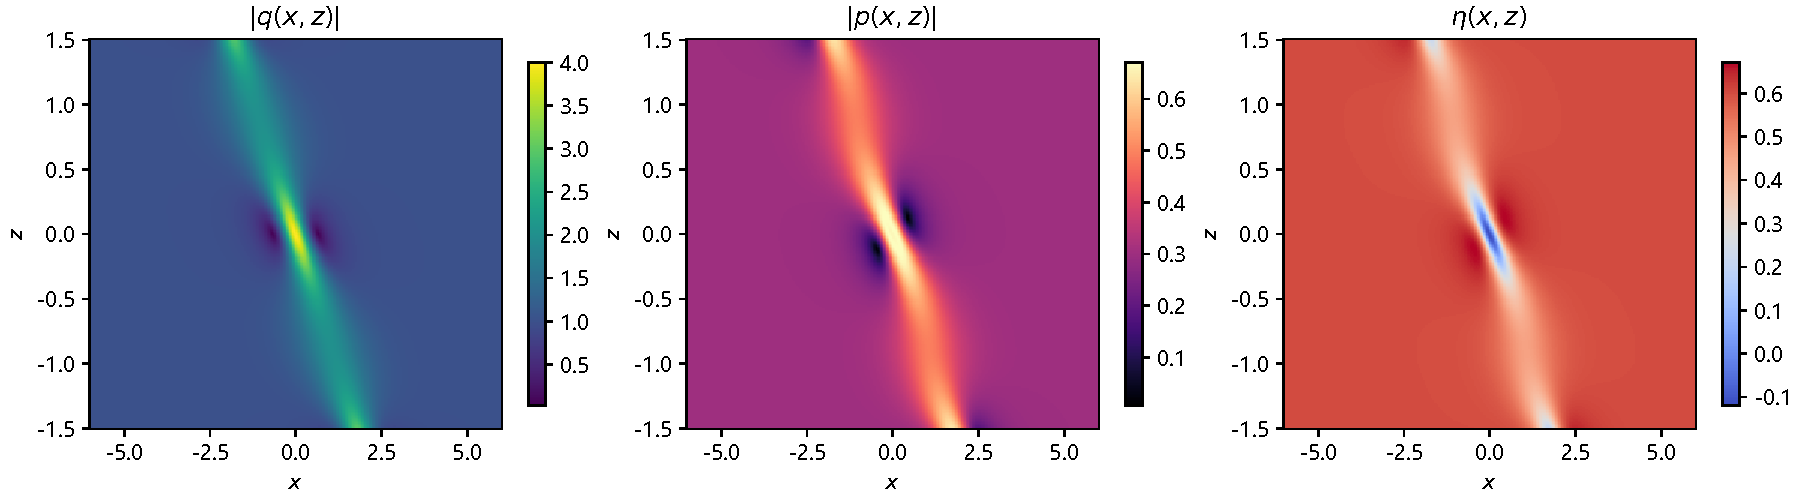
\includegraphics[width=\textwidth]{figures/one-soliton-fields.pdf}
\caption{一组四点谱轨道的三场图像。$Q=1,a=2,\eta_0=0.6,\alpha=1,\beta=0.1,b=1.5$；颜色分别表示 $|q|,|p|,\eta$。纵轴为传播变量 $z$，横轴为推迟时间 $x$。}
\label{fig:one}
\end{figure}
\begin{figure}[htbp]
\centering
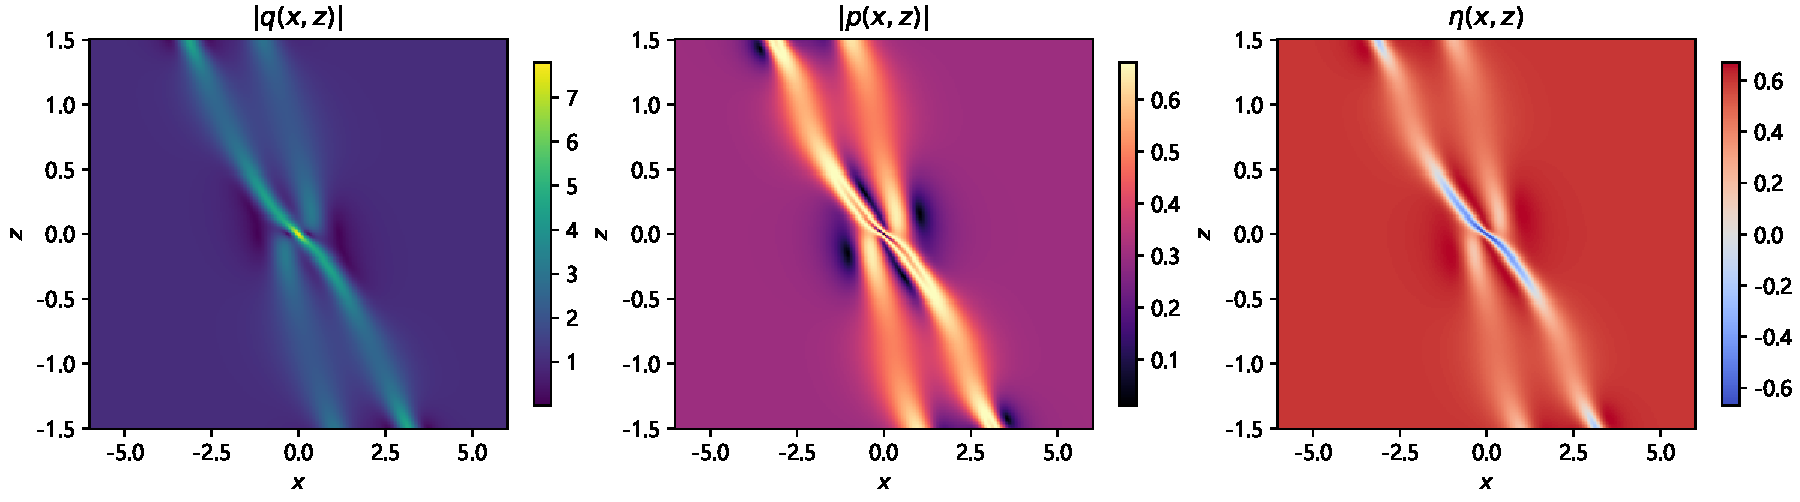
\includegraphics[width=\textwidth]{figures/two-soliton-fields.pdf}
\caption{同一背景下二次 dressing，谱点为 $1.5\ii,1.9\ii$。两个种子常向量均为 $(1,1)^{\mathsf T}$，三场由式 \eqref{eq:Nrecursion}--\eqref{eq:Nmedium} 递推得到。}
\label{fig:two}
\end{figure}

\chapter{总结与进一步研究}\label{ch:conclusion}
本章对定理 \ref{thm:direct-HMB} 的一轨道解进行数值求值, 展示三个场的空间分布及传播特征. 所用场值均由无反射留数系统求出, 光场和介质分别按 \eqref{eq:qfinite}、\eqref{eq:RfromM} 重构.

\section{散射数据与三场分布}
取背景和离散参数
\begin{equation}\label{eq:numerical-parameters}
Q=1,\quad a=2,\quad\eta_0=0.6,\quad
\alpha=1,\quad\beta=0.1,\quad b=1.5,
\end{equation}
范数常数按式 \eqref{eq:onec} 确定. 对每个 $(x,z)$, 直接组装式 \eqref{eq:one-AB} 对应的四阶块系统, 用两个右端项求出两组正则列, 再由部分分式表示计算 $M$. 绘图采用双精度线性代数, 各行先作尺度平衡; 介质保留复数计算结果, 并在求值后检查 $\eta$ 的虚部.

图 \ref{fig:one} 在 $x\in\lbrack-6,6\rbrack$、$z\in\lbrack-1.5,1.5\rbrack$ 上使用 $401\times251$ 网格. 光场在非零背景上形成局域振荡结构, 极化与粒子数反转在相同区域发生变化. 参数 \eqref{eq:numerical-parameters} 下 Bloch 长度平方为 $0.45$, 网格最大偏差小于 $7.78\times10^{-16}$, $\eta$ 虚部的最大绝对值小于 $5.21\times10^{-16}$.
\begin{figure}[htbp]
\centering
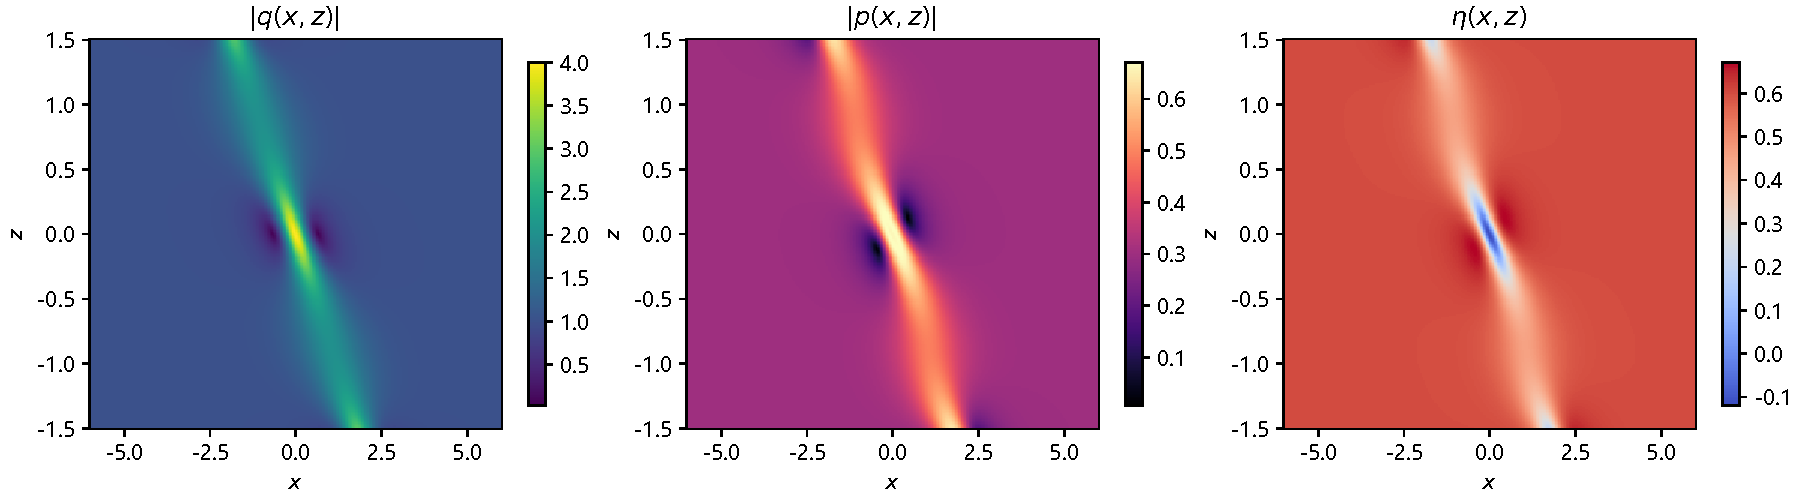
\includegraphics[width=\textwidth]{figures/one-soliton-fields.pdf}
\caption{由一轨道无反射留数系统重构的 $|q|,|p|,\eta$. 参数见 \eqref{eq:numerical-parameters}; 横轴为 $x$, 纵轴为 $z$.}
\label{fig:one}
\end{figure}

\section{传播速度与内部振荡}
由式 \eqref{eq:velocity}、\eqref{eq:frequency}, 上述参数给出
\[
A_b=-1.196,\qquad B_b=-1.572,\qquad
\kappa=\dfrac{\sqrt{5}}{2},\qquad T_z\approx1.78748466439.
\]
图 \ref{fig:dynamics} 左图比较 $z=0,\dfrac{T_z}{4},\dfrac{T_z}{2}$ 时的随动截面. 它们的差异来自式 \eqref{eq:hyperbolic-projector} 中的内部相位, 而局域化尺度由 $\kappa$ 决定. 右图在 $X=0$ 上改变 $\alpha$, 其余参数固定. 对应的解析频率和周期列于表 \ref{tab:periods}. 当 $\alpha=-0.048=-\dfrac{\eta_0}{a(a^2+b^2)}$ 时 $B_b=0$, 去相位三场为行波; 当 $B_b\ne0$ 时, 中心光场模随传播变量周期变化.
\begin{table}[htbp]
\centering
\caption{改变 $\alpha$ 时的随动内部频率与周期, 其余参数同 \eqref{eq:numerical-parameters}}
\label{tab:periods}
\begin{tabular}{cccc}
\toprule
$\alpha$ & $A_b$ & $B_b$ & $T_z$\\
\midrule
$-0.048$ & $-1.196$ & $0$ & 行波\\
$0.5$ & $-1.196$ & $-0.822$ & $3.41840132897$\\
$1$ & $-1.196$ & $-1.572$ & $1.78748466439$\\
\bottomrule
\end{tabular}
\end{table}
\begin{figure}[htbp]
\centering
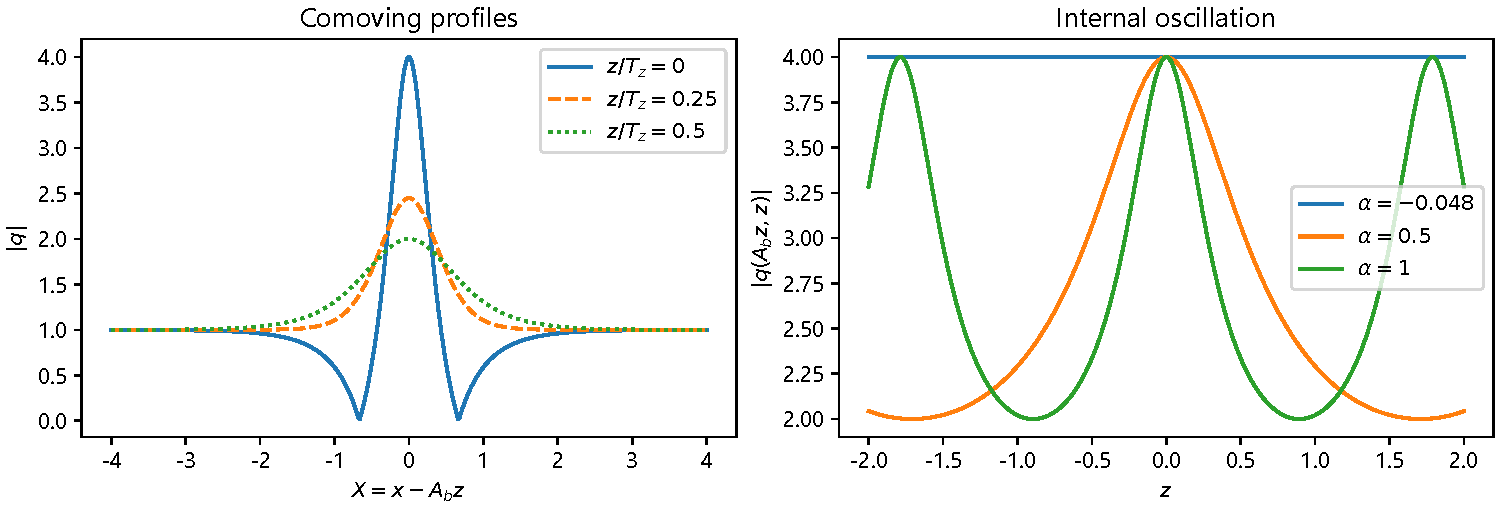
\includegraphics[width=\textwidth]{figures/one-soliton-dynamics.pdf}
\caption{一轨道光场的随动截面与内部振荡. 左图为基础参数下的三个截面, 右图为不同 $\alpha$ 下 $|q(A_bz,z)|$ 的变化.}
\label{fig:dynamics}
\end{figure}

参数 $\beta$ 出现在 $A_b$ 中, 不出现在 $B_b$ 中. 图 \ref{fig:velocity} 取 $\beta=0,0.15$, 对应速度分别为 $-0.096,-1.746$, 而两者均有 $B_b=-1.572$ 和相同的随动周期. 图中的虚线 $x=A_bz$ 给出随动坐标的中心轨迹. 这与命题 \ref{prop:wave-properties} 对传播平移和内部相位的分离一致.
\begin{figure}[htbp]
\centering
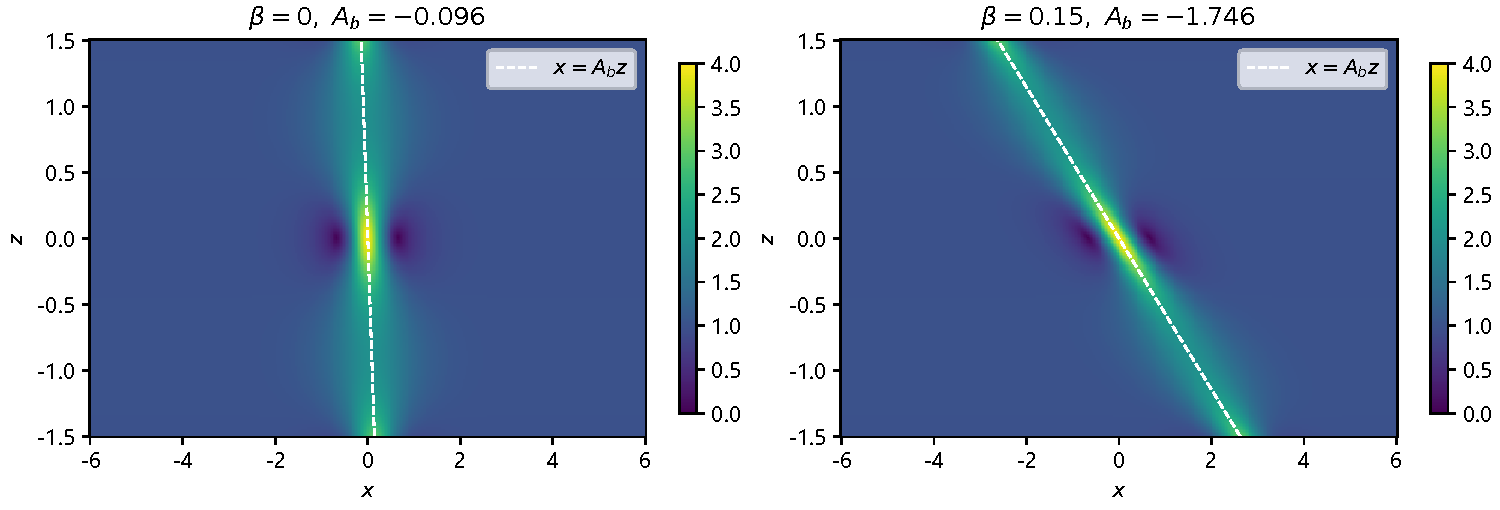
\includegraphics[width=\textwidth]{figures/one-soliton-velocity.pdf}
\caption{$\beta$ 对光场传播速度的影响. 两图分别取 $\beta=0,0.15$, 其余参数同 \eqref{eq:numerical-parameters}; 白色虚线为 $x=A_bz$.}
\label{fig:velocity}
\end{figure}

\section{精确参数例的代数检验}
作为一轨道公式的精确代数例, 取
\begin{equation}\label{eq:exactparams}
Q=1,\quad b=\dfrac{5}{4},\quad\kappa=\dfrac{3}{4},\quad
a=2,\quad\eta_0=\dfrac{3}{5},\quad\alpha=1,\quad\beta=\dfrac{1}{10}.
\end{equation}
此时 $h_0=\dfrac{1}{2}$, $F(\ii b)=-\dfrac{3321}{3560}-\dfrac{469\ii}{356}$. 令
$T=e^{2\operatorname{Re}s}>0$、$C=e^{2\ii\operatorname{Im}s}$, 则 $t=TC$、$\conj t=\dfrac{T}{C}$, 且
\[
\Delta_-=\dfrac{5}{4}(T^2+1)-T(C+C^{-1}).
\]
式 \eqref{eq:direct-vu1}--\eqref{eq:direct-vu2} 因而都是 $T,C$ 的有理式, 原方程可按
\[
\partial_x=2\kappa T\partial_T,\qquad
\partial_z=-2\kappa\operatorname{Re}F\,T\partial_T
-2\ii\kappa\operatorname{Im}F\,C\partial_C
\]
作精确检验. 代入式 \eqref{eq:finalfields} 后, 三条 PDE 的有理残差均为零, 且 $|p|^2+\eta^2=\dfrac{9}{20}$. 在 $T>0,|C|=1$ 上分母严格正, 清分母不引入额外解.


\section{高精度重构与方程残差}
对参数 \eqref{eq:numerical-parameters}, 采用 70 位十进制精度直接求解留数系统. 在五个时空点
\[
(-1.2,-0.35),\quad(0,0),\quad(0.37,0.21),\quad
(1.4,-0.1),\quad(2.3,0.6)
\]
对重构表达式作高精度微分, 得到表 \ref{tab:direct-residuals} 的最大绝对残差. 微分作用于线性系统的解及重构式, 三条 PDE 的右端用于计算残差. 矩阵检验另取三个普通谱点 $w=2.1+0.7\ii$、$0.3-0.2\ii$ 和 $1.2$.
\begin{table}[htbp]
\centering
\caption{五点采样下的独立重构检验, 数值均向上舍入}
\label{tab:direct-residuals}
\begin{tabular}{lc}
\toprule 检验对象 & 最大绝对误差\\\midrule
光场方程 & $1.87\times10^{-69}$\\
极化方程 & $8.26\times10^{-71}$\\
粒子数反转方程 & $1.50\times10^{-70}$\\
空间 Lax 方程 & $4.82\times10^{-70}$\\
传播 Lax 方程 & $1.95\times10^{-69}$\\
两个共振原像的介质重构 & $9.71\times10^{-72}$\\
Bloch 长度平方 & $9.07\times10^{-72}$\\
\bottomrule
\end{tabular}
\end{table}

同一组采样点上, 绘图实现与高精度实现的三个场最大差分别小于 $6.01\times10^{-16}$、$1.99\times10^{-16}$、$2.23\times10^{-16}$. 固定 $z=0.21$, 在 $x=\pm30$ 处检查式 \eqref{eq:targetboundary} 的三个端态, 最大误差小于 $5.02\times10^{-29}$. 留数、两种谱约化、行列式、归一化及分支点固定核也由同一矩阵逐项检验.

\appendix
\chapter{矩阵验算与复现实验}\label{app:checks}
\section{零曲率检查的展开顺序}
脚本 \texttt{verify\_symbolic.py} 将 $q,\conj q,p,\conj p,\eta$ 作为独立函数输入，避免计算机错误假设复函数的自变量为复数。先构造完整矩阵，再计算
$Z=U_z-V_x+UV-VU$，最后替换
\begin{align*}
q_z&=\ii\alpha(q_{xx}/2+q^2\conj q)
+\beta(q_{xxx}+6q\conj q\,q_x)+2p,\\
\conj{q}_z&=-\ii\alpha(\conj{q}_{xx}/2+\conj q^{\,2}q)
+\beta(\conj{q}_{xxx}+6q\conj q\,\conj{q}_x)+2\conj p,\\
p_x&=2\eta q-2\ii ap,\quad
\conj p_x=2\eta\conj q+2\ii a\conj p,\quad
\eta_x=-(\conj q p+q\conj p).
\end{align*}
输出 $Z$ 四个元素均为零。同时独立计算 $R_x-[U(a),R]$、Bloch 导数、背景时间矩阵以及 $U_\infty E+\ii\rho E\sg$。这些结果保存在
\texttt{evidence/symbolic-results.json}。它验证的是明确写出的代数表达，不依赖先前聊天中的任何计算结论。

\section{为什么空间谱并不决定介质}
仅由 $u=\ii M^{(1)}_{12}$ 得到光场后，介质方程在固定 $z$ 是沿 $x$ 的线性系统
$R_x=[U(a),R]$。若不给介质归一化，其解仍含任意常数矩阵：
\[
R(x,z)=\chi(x,a)C(z)\chi(x,a)^{-1}.
\]
Hermitian、迹零与 Bloch 长度约束只能限制 $C(z)$ 的形状和特征值，不能自动固定它的基底方向。本文通过相容端态确定
$C=\eta_0\rho(w_a)\sg/a$，才获得 \eqref{eq:RfromM}。所以只画出 $q$ 的轮廓，或只验证普通 Hirota 部分，均不能替代 HMB 三场解的构造。

\section{显式 RHP 验证的检查对象}
\texttt{verify\_rhp.py} 使用式 \eqref{eq:explicitM}，独立比较下列量：
\begin{align*}
&\det M-\left(1+\dfrac{Q^2}{w^2}\right),\\
&M(h(w))-M(w)\dfrac{\ii w}{Q}\sigma_1,\\
&M(w)-K\conj{M(\conj w)}K^{-1},\\
&M_x-(-\ii\lambda\sg+A(u))M-\ii\rho M\sg.
\end{align*}
留数通过有理分子的值除以 $\rho'(\zeta_j)$ 求得，而不是用极近点差商近似。然后与 $c_je^{2\ii\theta_j}M_2(\zeta_j)$ 比较。两个实共振原像分别代入 \eqref{eq:RfromM}，与独立 dressing 三场计算比较。这样的检查可以发现因子 2、共轭、换叶导数及相位旋转的符号错误。

\section{精确有理化为何有效}
对式 \eqref{eq:exactparams}，在真实的 $x,z$ 上 $T>0$ 且 $|C|=1$。脚本先把共轭列写成 $(T/C-1/2,\ 1-T/(2C))$，再在形式有理函数域 $\mathbb Q(\ii)(T,C)$ 中计算。若分子多项式恒等于零，限制到实际指数参数曲面后仍为零。分母中来自 $y^\dagger y$ 的因素在实际曲面上严格为正，共振分母也不为零，故清分母不引入实际奇点。

这比在若干网格上观察小残差强，但仍只直接覆盖该明确参数例。一般参数解的解析依据是原始 Darboux 定理和本文的端态、RHP 归一化计算。相关输出为
\texttt{evidence/exact-example-results.json}。

\section{数值实验的可重复性与局限}
数值残差脚本为 \texttt{verify\_solitons.py}，使用 mpmath 的 60 位任意精度求导。每条残差都从显式三场独立求导构造；二阶、三阶空间导数没有通过方程递推。保存的 JSON 包括参数、五个采样点、三条 PDE 的最大绝对残差、Bloch 偏差和左右端态误差。

绘图脚本采用 NumPy 双精度向量化，只用于生成图像；它不用于正文中的高精度残差声明。二者分开运行，避免把图形平滑性误当成方程成立的证据。

可复现顺序为：运行四个核验脚本，运行绘图脚本，然后执行 XeLaTeX、BibTeX、两次 XeLaTeX。具体命令、TeX 版本、构建日志和 PDF 页数记录在 \texttt{BUILD.md}。正文只引用已经实际生成的结果；后续若更改公式或参数，应重新运行对应检查并更新记录。

\backmatter
\bibliography{citelist}
\chapter{致谢}
待填写。本研究初稿使用计算机代数与高精度计算作为核验工具；数学论断的适用范围和未完成事项已在正文及研究状态报告中列出。
\end{document}
